% !TeX program = xelatex
% UIR 2; variant 33/73/11. Unzip the complete package before compiling.
% Compile twice: xelatex UIR2_Mikhailov_33-73-11.tex
% The calculation source is included from ../app/calculate_uir2.py.
\documentclass[a4paper,12pt]{article}
\usepackage{iftex}
\ifPDFTeX
  \usepackage[T2A]{fontenc}
  \usepackage[utf8]{inputenc}
  \usepackage[russian]{babel}
\else
  \usepackage{fontspec}
  \usepackage{polyglossia}
  \setdefaultlanguage{russian}
  \setotherlanguage{english}
  \IfFontExistsTF{Times New Roman}{%
    \setmainfont{Times New Roman}\newfontfamily\cyrillicfont{Times New Roman}}{%
    \IfFontExistsTF{NimbusRoman-Regular.otf}{%
      \setmainfont{NimbusRoman}[Extension=.otf,UprightFont=*-Regular,BoldFont=*-Bold,ItalicFont=*-Italic,BoldItalicFont=*-BoldItalic]
      \newfontfamily\cyrillicfont{NimbusRoman}[Extension=.otf,UprightFont=*-Regular,BoldFont=*-Bold,ItalicFont=*-Italic,BoldItalicFont=*-BoldItalic]
    }{\setmainfont{DejaVu Serif}\newfontfamily\cyrillicfont{DejaVu Serif}}}
  \setsansfont{DejaVu Sans}
  \newfontfamily\cyrillicfontsf{DejaVu Sans}
  \setmonofont{DejaVu Sans Mono}
  \newfontfamily\cyrillicfonttt{DejaVu Sans Mono}
\fi
\usepackage{amsmath,amssymb,amsfonts}
\usepackage{graphicx,geometry,listings,xcolor,hyperref,float,booktabs}
\usepackage{longtable,array,tabularx,caption}
\usepackage{tikz,pgfplots}
\usetikzlibrary{arrows.meta,fit,positioning}
\pgfplotsset{compat=1.18}
\geometry{left=2cm,right=1.5cm,top=2cm,bottom=2cm}
\hypersetup{unicode=true,colorlinks=true,linkcolor=black,citecolor=black,urlcolor=blue!60!black,
 pdftitle={УИР 2. Марковские модели СМО. Вариант 33/73/11},pdfauthor={Михайлов Петр Сергеевич}}
\captionsetup{font=small,labelsep=period}
\setlength{\parindent}{1.25cm}
\setlength{\parskip}{.2em}
\linespread{1.05}
\raggedbottom
\setcounter{tocdepth}{2}
\setlength{\emergencystretch}{2em}
\tolerance=3000
\newcommand{\sysone}{СИСТЕМА\_1}
\newcommand{\systwo}{СИСТЕМА\_2}
\newcommand{\ind}{\mathbf1}
\newcommand{\secunit}{\,\text{с}^{-1}}
\lstdefinestyle{mypython}{language=Python,basicstyle=\ttfamily\scriptsize,
 keywordstyle=\color{blue!65!black}\bfseries,stringstyle=\color{red!65!black},
 commentstyle=\color{green!35!black},numbers=left,numberstyle=\tiny\color{gray},
 stepnumber=1,numbersep=7pt,showstringspaces=false,tabsize=4,frame=single,
 breaklines=true,breakatwhitespace=false,columns=fullflexible,keepspaces=true,
 xleftmargin=14pt,framexleftmargin=10pt,backgroundcolor=\color{gray!3}}
\lstset{style=mypython}

\begin{document}
\begin{titlepage}
\centering
{\fontsize{11}{13}\selectfont\textbf{Министерство науки и высшего образования Российской Федерации}}\\
{\fontsize{7}{10}\selectfont ФЕДЕРАЛЬНОЕ ГОСУДАРСТВЕННОЕ АВТОНОМНОЕ ОБРАЗОВАТЕЛЬНОЕ УЧРЕЖДЕНИЕ ВЫСШЕГО ОБРАЗОВАНИЯ}\\
\vspace{.2cm}
{\fontsize{14}{17}\selectfont\textbf{«НАЦИОНАЛЬНЫЙ ИССЛЕДОВАТЕЛЬСКИЙ УНИВЕРСИТЕТ ИТМО»}}
\vspace{1cm}

{\fontsize{12}{14}\selectfont\textbf{Факультет программной инженерии и компьютерной техники}}
\vspace{1cm}

{\fontsize{12}{14}\selectfont\textbf{Дисциплина: Моделирование}}
\vspace*{\fill}

{\fontsize{18}{22}\selectfont\textbf{УЧЕБНО-ИССЛЕДОВАТЕЛЬСКАЯ\\РАБОТА №2}}\\
\vspace{.5cm}
{\fontsize{14}{17}\selectfont\textbf{по теме: «Марковские модели систем\\массового обслуживания»}}
\vspace{1.5cm}

{\fontsize{12}{14}\selectfont\textbf{Вариант: 33/73/11}}
\vspace{1.5cm}
\begin{flushright}
\fontsize{12}{14}\selectfont
Выполнил:\\
Михайлов Петр Сергеевич\\
Группа: P3311\\[1em]
Преподаватель:\\
Тропченко Андрей Александрович
\end{flushright}
\vfill
{\fontsize{12}{14}\selectfont Санкт-Петербург, 2026}
\end{titlepage}
\setcounter{page}{2}
{\small\setlength{\parskip}{0pt}\tableofcontents}
\newpage

\section{Цель и задачи работы}
\textbf{Цель работы} --- изучить метод марковских случайных процессов с непрерывным временем и применить его для исследования систем массового обслуживания (СМО) с однородным потоком заявок.

Для достижения цели необходимо описать две заданные системы, закодировать их состояния, построить размеченные графы переходов и матрицы интенсивностей, найти стационарные вероятности и рассчитать через них характеристики обслуживания. Затем требуется проверить результаты фундаментальными зависимостями, исследовать влияние интенсивности входного потока и выбрать лучшую организацию системы по критерию варианта.

\section{Постановка задачи и исходные данные}
Номер варианта: $N_1/N_2/N_G=33/73/11$. По таблице~1 задания~\cite{task} выбираются структуры систем, по таблице~2 --- параметры нагрузки. Поскольку $33+73=106$ --- чётное число, критерий определяется строкой $N_2=73$: \textbf{(в) максимальная загрузка системы}.

\begin{table}[H]
\centering\caption{Исходные данные варианта 33/73/11}\label{tab:input}
\begin{tabularx}{\linewidth}{@{}>{\raggedright\arraybackslash}p{5.3cm}>{\raggedright\arraybackslash}X>{\raggedright\arraybackslash}X@{}}\toprule
Параметр & \sysone & \systwo\\\midrule
Вариант структуры & 33 & 73\\
Число приборов $c$ & 2 & 3\\
Ёмкости накопителей & $2/1$ & $1/0/1$\\
Максимум заявок у приборов $K_i$ & $(3,2)$ & $(2,1,2)$\\
Закон обслуживания & экспоненциальный в обоих приборах & Эрланга $E_2$ в П1; экспоненциальный в П2 и П3\\
Вероятности направления $q_i$ & $(0{,}75;0{,}25)$ & $(0{,}75;0{,}20;0{,}05)$\\
Интенсивности $\lambda_i$, $\text{с}^{-1}$ & $(0{,}45;0{,}15)$ & $(0{,}45;0{,}12;0{,}03)$\\
Общий входной поток $\lambda$ & \multicolumn{2}{l}{$0{,}6\secunit$}\\
Среднее обслуживание $b$ & \multicolumn{2}{l}{$5$ с в каждом приборе обеих систем}\\
Интенсивность экспоненциального обслуживания $\mu=1/b$ & \multicolumn{2}{l}{$0{,}2\secunit$}\\
Критерий эффективности & \multicolumn{2}{l}{максимум суммарной загрузки $R$}\\\bottomrule
\end{tabularx}
\end{table}

У двухприборной системы вероятность направления ко второму прибору равна сумме двух последних вероятностей таблицы~2: $q_2=0{,}20+0{,}05=0{,}25$. Ёмкость накопителя \emph{не включает} обслуживаемую заявку, поэтому $K_i=r_i+1$, где $r_i$ --- число мест ожидания.

Обозначение $3(E_2)$ по заданию относится к \emph{одному} из трёх приборов. Выбран прибор П1, принимающий наибольшую долю входного потока. В остальных приборах сохраняется экспоненциальное обслуживание. В основных расчётах и при варьировании $\lambda$ этот выбор фиксирован. Влияние выбора прибора отдельно проверено в разделе~\ref{sec:placement}.

\section{Описание систем и способ расчёта}
Входной поток --- простейший. Каждая заявка независимо направляется к прибору П$i$ с вероятностью $q_i$, поэтому отдельные входные потоки являются независимыми пуассоновскими потоками с $\lambda_i=q_i\lambda$. Если выбранный прибор свободен, обслуживание начинается сразу; иначе заявка занимает свободное место его накопителя. При заполненном накопителе она теряется. Перенаправления к другим приборам нет.

Дисциплина очереди --- FIFO; обслуживание не прерывается. Длительности обслуживания разных заявок и входные потоки независимы. Потерянные заявки не возвращаются. Мгновенная передача очередной заявки из накопителя в прибор не требует отдельного состояния.

\subsection{Фазовое представление распределения Эрланга}
В П1 второй системы время обслуживания является суммой двух независимых экспоненциальных фаз:
\[
B=B^{(1)}+B^{(2)},\qquad B^{(f)}\sim\operatorname{Exp}(\nu),\qquad
\nu=\frac{2}{b}=0{,}4\secunit.
\]
Следовательно, $\mathsf E B=2/\nu=5$ с, $\operatorname{Var}B=2/\nu^2=12{,}5\ \text{с}^2$, коэффициент вариации равен $1/\sqrt2$. Две фазы выполняются \emph{последовательно одним прибором}: одновременно две заявки в нём не обслуживаются. Переход между фазами не означает уход заявки. Включение номера текущей фазы в состояние делает процесс марковским~\cite{theory}.

\subsection{Вычислительный метод и воспроизводимость}
Обе полные модели рассчитаны в программе MARK (WinMark): введены элементы и матрицы интенсивностей, получены стационарные вероятности, вычислены характеристики по 24 формулам для \sysone\ и 32 формулам для \systwo, выполнено варьирование интенсивностей и построены графики. Снимки окон программы, результаты сверки и экспортированные графики приведены в разделе~\ref{sec:winmark}; полные HTML-отчёты входят в электронное приложение~\cite{mark1,mark2}.

Независимая программа на Python 3.12.14 со стандартной библиотекой строит генераторы и решает стационарные уравнения методом Гаусса с выбором главного элемента. Времена вычисляются прямым усреднением условных времён по состояниям. Программа используется для проверки WinMark, контрольных экспериментов и уточнения точки пересечения кривых. Имитационное моделирование и оценивание по случайным выборкам не применяются. Исходный код и фактический протокол приведены в приложениях~\ref{app:code} и~\ref{app:log}.

Полные модели содержат 12 и 30 состояний. На странице~7 задания допускается обоснованное изменение структуры, если состояний больше 20. В данном расчёте WinMark обрабатывает все 30 состояний: это подтверждается матрицей и вероятностями в \texttt{report\_system2.html} и файлом \texttt{system2\_73.mrk}. Поэтому число приборов и ёмкости накопителей сохранены точно по варианту; сокращённая модель не строилась.

Исходный код, модели WinMark, результаты расчётов и материалы отчёта размещены в репозитории:
\href{https://github.com/Axe-On-You/Modeling/tree/main/\%D0\%9B\%D0\%B0\%D0\%B1\%D0\%BE\%D1\%80\%D0\%B0\%D1\%82\%D0\%BE\%D1\%80\%D0\%BD\%D0\%B0\%D1\%8F\%202}
{Axe-On-You/Modeling, папка «Лабораторная 2»}.

\section{Марковские модели исследуемых систем}
\subsection{Кодирование и перечень состояний}
Для \sysone\ состояние $(n_1,n_2)$ задаёт число заявок в каждом узле вместе с обслуживаемой:
\[
n_1\in\{0,1,2,3\},\qquad n_2\in\{0,1,2\},\qquad
E_{3n_1+n_2}=(n_1,n_2).
\]
Всего $4\cdot3=12$ состояний, от $E_0=(0,0)$ до $E_{11}=(3,2)$.

Для \systwo\ локальное состояние П1 кодируется символом
\[
a\in\{0,1_1,1_2,2_1,2_2\}.
\]
Здесь $0$ означает свободный прибор, $n_f$ --- $n$ заявок в узле и обслуживание текущей заявки в фазе $f$. Например, $2_2$ означает одну заявку на второй фазе обслуживания и одну в накопителе. Пусть $j(a)=0,1,2,3,4$ в указанном порядке. Тогда
\[
E_{6j(a)+3n_2+n_3}=(a,n_2,n_3),\qquad
n_2\in\{0,1\},\quad n_3\in\{0,1,2\}.
\]
Всего $5\cdot2\cdot3=30$ состояний. Например, $E_8=(1_1,0,2)$, $E_{29}=(2_2,1,2)$. Полный перечень \emph{всех} состояний обеих систем с вероятностями приведён в таблице~\ref{tab:prob}.

\subsection{Размеченные графы переходов}
В первой системе поступление к П$i$ увеличивает $n_i$ на единицу с интенсивностью $\lambda_i$, если $n_i<K_i$. Завершение обслуживания уменьшает $n_i$ на единицу с интенсивностью $\mu$, если $n_i>0$. Одновременное изменение двух координат не допускается. Полный граф представлен на рисунке~\ref{fig:graph1}.

\begin{figure}[H]\centering
\begin{tikzpicture}[>=Stealth,font=\small,state/.style={draw,circle,minimum size=12mm,inner sep=1pt,align=center},every edge/.style={->}]
\node[state] (s0) at (0.0,-0.0) {$E_{0}$\\[-1pt]{\scriptsize $(0,0)$}};
\node[state] (s1) at (0.0,-2.0) {$E_{1}$\\[-1pt]{\scriptsize $(0,1)$}};
\node[state] (s2) at (0.0,-4.0) {$E_{2}$\\[-1pt]{\scriptsize $(0,2)$}};
\node[state] (s3) at (3.1,-0.0) {$E_{3}$\\[-1pt]{\scriptsize $(1,0)$}};
\node[state] (s4) at (3.1,-2.0) {$E_{4}$\\[-1pt]{\scriptsize $(1,1)$}};
\node[state] (s5) at (3.1,-4.0) {$E_{5}$\\[-1pt]{\scriptsize $(1,2)$}};
\node[state] (s6) at (6.2,-0.0) {$E_{6}$\\[-1pt]{\scriptsize $(2,0)$}};
\node[state] (s7) at (6.2,-2.0) {$E_{7}$\\[-1pt]{\scriptsize $(2,1)$}};
\node[state] (s8) at (6.2,-4.0) {$E_{8}$\\[-1pt]{\scriptsize $(2,2)$}};
\node[state] (s9) at (9.3,-0.0) {$E_{9}$\\[-1pt]{\scriptsize $(3,0)$}};
\node[state] (s10) at (9.3,-2.0) {$E_{10}$\\[-1pt]{\scriptsize $(3,1)$}};
\node[state] (s11) at (9.3,-4.0) {$E_{11}$\\[-1pt]{\scriptsize $(3,2)$}};
\draw[->] (s0) to[bend left=12] node[above] {$\lambda_1$} (s3);
\draw[->] (s3) to[bend left=12] node[below] {$\mu$} (s0);
\draw[->] (s0) to[bend left=14] node[right] {$\lambda_2$} (s1);
\draw[->] (s1) to[bend left=14] node[left] {$\mu$} (s0);
\draw[->] (s1) to[bend left=12] node[above] {$\lambda_1$} (s4);
\draw[->] (s4) to[bend left=12] node[below] {$\mu$} (s1);
\draw[->] (s1) to[bend left=14] node[right] {$\lambda_2$} (s2);
\draw[->] (s2) to[bend left=14] node[left] {$\mu$} (s1);
\draw[->] (s2) to[bend left=12] node[above] {$\lambda_1$} (s5);
\draw[->] (s5) to[bend left=12] node[below] {$\mu$} (s2);
\draw[->] (s3) to[bend left=12] node[above] {$\lambda_1$} (s6);
\draw[->] (s6) to[bend left=12] node[below] {$\mu$} (s3);
\draw[->] (s3) to[bend left=14] node[right] {$\lambda_2$} (s4);
\draw[->] (s4) to[bend left=14] node[left] {$\mu$} (s3);
\draw[->] (s4) to[bend left=12] node[above] {$\lambda_1$} (s7);
\draw[->] (s7) to[bend left=12] node[below] {$\mu$} (s4);
\draw[->] (s4) to[bend left=14] node[right] {$\lambda_2$} (s5);
\draw[->] (s5) to[bend left=14] node[left] {$\mu$} (s4);
\draw[->] (s5) to[bend left=12] node[above] {$\lambda_1$} (s8);
\draw[->] (s8) to[bend left=12] node[below] {$\mu$} (s5);
\draw[->] (s6) to[bend left=12] node[above] {$\lambda_1$} (s9);
\draw[->] (s9) to[bend left=12] node[below] {$\mu$} (s6);
\draw[->] (s6) to[bend left=14] node[right] {$\lambda_2$} (s7);
\draw[->] (s7) to[bend left=14] node[left] {$\mu$} (s6);
\draw[->] (s7) to[bend left=12] node[above] {$\lambda_1$} (s10);
\draw[->] (s10) to[bend left=12] node[below] {$\mu$} (s7);
\draw[->] (s7) to[bend left=14] node[right] {$\lambda_2$} (s8);
\draw[->] (s8) to[bend left=14] node[left] {$\mu$} (s7);
\draw[->] (s8) to[bend left=12] node[above] {$\lambda_1$} (s11);
\draw[->] (s11) to[bend left=12] node[below] {$\mu$} (s8);
\draw[->] (s9) to[bend left=14] node[right] {$\lambda_2$} (s10);
\draw[->] (s10) to[bend left=14] node[left] {$\mu$} (s9);
\draw[->] (s10) to[bend left=14] node[right] {$\lambda_2$} (s11);
\draw[->] (s11) to[bend left=14] node[left] {$\mu$} (s10);
\end{tikzpicture}
\caption{Размеченный граф \sysone: $\lambda_1=0{,}45$, $\lambda_2=0{,}15$, $\mu=0{,}2\secunit$.}\label{fig:graph1}
\end{figure}

Для П1 второй системы локальные переходы имеют вид
\[
0\xrightarrow{\lambda_1}1_1,\quad
1_1\xrightarrow{\nu}1_2,\quad
1_2\xrightarrow{\nu}0,\quad
1_1\xrightarrow{\lambda_1}2_1,\quad
1_2\xrightarrow{\lambda_1}2_2,\quad
2_1\xrightarrow{\nu}2_2,\quad
2_2\xrightarrow{\nu}1_1.
\]
Последняя дуга означает завершение обслуживания текущей заявки и начало обслуживания ожидающей в первой фазе. Поступление в состояниях $2_1,2_2$ теряется. У П2 и П3 действуют обычные экспоненциальные переходы при своих ограничениях ёмкости.

\begin{figure}[H]\centering
\resizebox{.98\linewidth}{!}{%
\begin{tikzpicture}[>=Stealth,font=\scriptsize,smallstate/.style={draw,circle,minimum size=7mm,inner sep=1pt,fill=white}]
\begin{scope}[shift={(0.0,-0.0)}]
\node[smallstate] (e0) at (-1.05,0) {$E_{0}$};
\node[smallstate] (e6) at (0.0,0.85) {$E_{6}$};
\node[smallstate] (e12) at (0.0,-0.85) {$E_{12}$};
\node[smallstate] (e18) at (1.35,0.85) {$E_{18}$};
\node[smallstate] (e24) at (1.35,-0.85) {$E_{24}$};
\draw[->] (e0) -- node[above left,fill=white,inner sep=.6pt] {$\lambda_1$} (e6);
\draw[->] (e6) -- node[left,fill=white,inner sep=.6pt] {$\nu$} (e12);
\draw[->] (e12) -- node[below left,fill=white,inner sep=.6pt] {$\nu$} (e0);
\draw[->] (e6) -- node[above,fill=white,inner sep=.6pt] {$\lambda_1$} (e18);
\draw[->] (e12) -- node[below,fill=white,inner sep=.6pt] {$\lambda_1$} (e24);
\draw[->] (e18) -- node[right,fill=white,inner sep=.6pt] {$\nu$} (e24);
\draw[->] (e24) -- node[above right,fill=white,inner sep=.6pt] {$\nu$} (e6);
\node[draw,rounded corners=3pt,fit=(e0)(e6)(e12)(e18)(e24),inner sep=10pt] (g0) {};
\node[font=\scriptsize,anchor=north,inner sep=1pt] at (g0.north) {$n_2=0,\ n_3=0$};
\end{scope}
\begin{scope}[shift={(5.1,-0.0)}]
\node[smallstate] (e1) at (-1.05,0) {$E_{1}$};
\node[smallstate] (e7) at (0.0,0.85) {$E_{7}$};
\node[smallstate] (e13) at (0.0,-0.85) {$E_{13}$};
\node[smallstate] (e19) at (1.35,0.85) {$E_{19}$};
\node[smallstate] (e25) at (1.35,-0.85) {$E_{25}$};
\draw[->] (e1) -- node[above left,fill=white,inner sep=.6pt] {$\lambda_1$} (e7);
\draw[->] (e7) -- node[left,fill=white,inner sep=.6pt] {$\nu$} (e13);
\draw[->] (e13) -- node[below left,fill=white,inner sep=.6pt] {$\nu$} (e1);
\draw[->] (e7) -- node[above,fill=white,inner sep=.6pt] {$\lambda_1$} (e19);
\draw[->] (e13) -- node[below,fill=white,inner sep=.6pt] {$\lambda_1$} (e25);
\draw[->] (e19) -- node[right,fill=white,inner sep=.6pt] {$\nu$} (e25);
\draw[->] (e25) -- node[above right,fill=white,inner sep=.6pt] {$\nu$} (e7);
\node[draw,rounded corners=3pt,fit=(e1)(e7)(e13)(e19)(e25),inner sep=10pt] (g1) {};
\node[font=\scriptsize,anchor=north,inner sep=1pt] at (g1.north) {$n_2=0,\ n_3=1$};
\end{scope}
\begin{scope}[shift={(10.2,-0.0)}]
\node[smallstate] (e2) at (-1.05,0) {$E_{2}$};
\node[smallstate] (e8) at (0.0,0.85) {$E_{8}$};
\node[smallstate] (e14) at (0.0,-0.85) {$E_{14}$};
\node[smallstate] (e20) at (1.35,0.85) {$E_{20}$};
\node[smallstate] (e26) at (1.35,-0.85) {$E_{26}$};
\draw[->] (e2) -- node[above left,fill=white,inner sep=.6pt] {$\lambda_1$} (e8);
\draw[->] (e8) -- node[left,fill=white,inner sep=.6pt] {$\nu$} (e14);
\draw[->] (e14) -- node[below left,fill=white,inner sep=.6pt] {$\nu$} (e2);
\draw[->] (e8) -- node[above,fill=white,inner sep=.6pt] {$\lambda_1$} (e20);
\draw[->] (e14) -- node[below,fill=white,inner sep=.6pt] {$\lambda_1$} (e26);
\draw[->] (e20) -- node[right,fill=white,inner sep=.6pt] {$\nu$} (e26);
\draw[->] (e26) -- node[above right,fill=white,inner sep=.6pt] {$\nu$} (e8);
\node[draw,rounded corners=3pt,fit=(e2)(e8)(e14)(e20)(e26),inner sep=10pt] (g2) {};
\node[font=\scriptsize,anchor=north,inner sep=1pt] at (g2.north) {$n_2=0,\ n_3=2$};
\end{scope}
\begin{scope}[shift={(0.0,-4.7)}]
\node[smallstate] (e3) at (-1.05,0) {$E_{3}$};
\node[smallstate] (e9) at (0.0,0.85) {$E_{9}$};
\node[smallstate] (e15) at (0.0,-0.85) {$E_{15}$};
\node[smallstate] (e21) at (1.35,0.85) {$E_{21}$};
\node[smallstate] (e27) at (1.35,-0.85) {$E_{27}$};
\draw[->] (e3) -- node[above left,fill=white,inner sep=.6pt] {$\lambda_1$} (e9);
\draw[->] (e9) -- node[left,fill=white,inner sep=.6pt] {$\nu$} (e15);
\draw[->] (e15) -- node[below left,fill=white,inner sep=.6pt] {$\nu$} (e3);
\draw[->] (e9) -- node[above,fill=white,inner sep=.6pt] {$\lambda_1$} (e21);
\draw[->] (e15) -- node[below,fill=white,inner sep=.6pt] {$\lambda_1$} (e27);
\draw[->] (e21) -- node[right,fill=white,inner sep=.6pt] {$\nu$} (e27);
\draw[->] (e27) -- node[above right,fill=white,inner sep=.6pt] {$\nu$} (e9);
\node[draw,rounded corners=3pt,fit=(e3)(e9)(e15)(e21)(e27),inner sep=10pt] (g3) {};
\node[font=\scriptsize,anchor=north,inner sep=1pt] at (g3.north) {$n_2=1,\ n_3=0$};
\end{scope}
\begin{scope}[shift={(5.1,-4.7)}]
\node[smallstate] (e4) at (-1.05,0) {$E_{4}$};
\node[smallstate] (e10) at (0.0,0.85) {$E_{10}$};
\node[smallstate] (e16) at (0.0,-0.85) {$E_{16}$};
\node[smallstate] (e22) at (1.35,0.85) {$E_{22}$};
\node[smallstate] (e28) at (1.35,-0.85) {$E_{28}$};
\draw[->] (e4) -- node[above left,fill=white,inner sep=.6pt] {$\lambda_1$} (e10);
\draw[->] (e10) -- node[left,fill=white,inner sep=.6pt] {$\nu$} (e16);
\draw[->] (e16) -- node[below left,fill=white,inner sep=.6pt] {$\nu$} (e4);
\draw[->] (e10) -- node[above,fill=white,inner sep=.6pt] {$\lambda_1$} (e22);
\draw[->] (e16) -- node[below,fill=white,inner sep=.6pt] {$\lambda_1$} (e28);
\draw[->] (e22) -- node[right,fill=white,inner sep=.6pt] {$\nu$} (e28);
\draw[->] (e28) -- node[above right,fill=white,inner sep=.6pt] {$\nu$} (e10);
\node[draw,rounded corners=3pt,fit=(e4)(e10)(e16)(e22)(e28),inner sep=10pt] (g4) {};
\node[font=\scriptsize,anchor=north,inner sep=1pt] at (g4.north) {$n_2=1,\ n_3=1$};
\end{scope}
\begin{scope}[shift={(10.2,-4.7)}]
\node[smallstate] (e5) at (-1.05,0) {$E_{5}$};
\node[smallstate] (e11) at (0.0,0.85) {$E_{11}$};
\node[smallstate] (e17) at (0.0,-0.85) {$E_{17}$};
\node[smallstate] (e23) at (1.35,0.85) {$E_{23}$};
\node[smallstate] (e29) at (1.35,-0.85) {$E_{29}$};
\draw[->] (e5) -- node[above left,fill=white,inner sep=.6pt] {$\lambda_1$} (e11);
\draw[->] (e11) -- node[left,fill=white,inner sep=.6pt] {$\nu$} (e17);
\draw[->] (e17) -- node[below left,fill=white,inner sep=.6pt] {$\nu$} (e5);
\draw[->] (e11) -- node[above,fill=white,inner sep=.6pt] {$\lambda_1$} (e23);
\draw[->] (e17) -- node[below,fill=white,inner sep=.6pt] {$\lambda_1$} (e29);
\draw[->] (e23) -- node[right,fill=white,inner sep=.6pt] {$\nu$} (e29);
\draw[->] (e29) -- node[above right,fill=white,inner sep=.6pt] {$\nu$} (e11);
\node[draw,rounded corners=3pt,fit=(e5)(e11)(e17)(e23)(e29),inner sep=10pt] (g5) {};
\node[font=\scriptsize,anchor=north,inner sep=1pt] at (g5.north) {$n_2=1,\ n_3=2$};
\end{scope}
\draw[->,thick] (g0.east) to[bend left=16] node[above] {$\lambda_3$} (g1.west);
\draw[->,thick] (g1.west) to[bend left=16] node[below] {$\mu$} (g0.east);
\draw[->,thick] (g0.south) to[bend left=12] node[right] {$\lambda_2$} (g3.north);
\draw[->,thick] (g3.north) to[bend left=12] node[left] {$\mu$} (g0.south);
\draw[->,thick] (g1.east) to[bend left=16] node[above] {$\lambda_3$} (g2.west);
\draw[->,thick] (g2.west) to[bend left=16] node[below] {$\mu$} (g1.east);
\draw[->,thick] (g1.south) to[bend left=12] node[right] {$\lambda_2$} (g4.north);
\draw[->,thick] (g4.north) to[bend left=12] node[left] {$\mu$} (g1.south);
\draw[->,thick] (g2.south) to[bend left=12] node[right] {$\lambda_2$} (g5.north);
\draw[->,thick] (g5.north) to[bend left=12] node[left] {$\mu$} (g2.south);
\draw[->,thick] (g3.east) to[bend left=16] node[above] {$\lambda_3$} (g4.west);
\draw[->,thick] (g4.west) to[bend left=16] node[below] {$\mu$} (g3.east);
\draw[->,thick] (g4.east) to[bend left=16] node[above] {$\lambda_3$} (g5.west);
\draw[->,thick] (g5.west) to[bend left=16] node[below] {$\mu$} (g4.east);
\end{tikzpicture}}
\caption{Полный размеченный граф \systwo\ в блочном представлении: показаны все 30 вершин. Внутри блоков $\lambda_1=0{,}45$, $\nu=0{,}4$; между блоками $\lambda_2=0{,}12$, $\lambda_3=0{,}03$, $\mu=0{,}2\secunit$.}\label{fig:graph2}
\end{figure}

Каждая стрелка между блоками рисунка~\ref{fig:graph2} обозначает пять дуг между \emph{соответствующими} вершинами с одинаковым состоянием $a$ прибора П1. Точная расшифровка:
\[
\begin{aligned}
E_{6j+3n_2+n_3}&\xrightarrow{\lambda_3}E_{6j+3n_2+n_3+1},&& n_3<2,\\
E_{6j+3n_2+n_3}&\xrightarrow{\mu}E_{6j+3n_2+n_3-1},&& n_3>0,\\
E_{6j+n_3}&\xrightarrow{\lambda_2}E_{6j+3+n_3},&& n_2=0,\\
E_{6j+3+n_3}&\xrightarrow{\mu}E_{6j+n_3},&& n_2=1,
\end{aligned}\qquad j=0,\ldots,4.
\]
Таким образом, блочное представление задаёт все дуги исходной модели и не объединяет различные марковские состояния.

Отказы не меняют состояние, поэтому отдельные петли отказов в графах и положительные слагаемые от отказов на диагонали генератора не вводятся. Потери учитываются отдельно через вероятности заполнения соответствующих узлов.

\subsection{Матрицы интенсивностей переходов}
Используется строковое соглашение: $g_{ij}$ --- интенсивность перехода из $E_i$ в $E_j$, $i\ne j$, а $g_{ii}=-\sum_{j\ne i}g_{ij}$. Все интенсивности далее измеряются в $\text{с}^{-1}$.

Полная численная матрица первой системы:
\begin{equation}\label{eq:q1}
\resizebox{\linewidth}{!}{$G_1=\left(\begin{array}{rrrrrrrrrrrr}
-0{,}60 & 0{,}15 & 0 & 0{,}45 & 0 & 0 & 0 & 0 & 0 & 0 & 0 & 0 \\0{,}20 & -0{,}80 & 0{,}15 & 0 & 0{,}45 & 0 & 0 & 0 & 0 & 0 & 0 & 0 \\0 & 0{,}20 & -0{,}65 & 0 & 0 & 0{,}45 & 0 & 0 & 0 & 0 & 0 & 0 \\0{,}20 & 0 & 0 & -0{,}80 & 0{,}15 & 0 & 0{,}45 & 0 & 0 & 0 & 0 & 0 \\0 & 0{,}20 & 0 & 0{,}20 & -1{,}00 & 0{,}15 & 0 & 0{,}45 & 0 & 0 & 0 & 0 \\0 & 0 & 0{,}20 & 0 & 0{,}20 & -0{,}85 & 0 & 0 & 0{,}45 & 0 & 0 & 0 \\0 & 0 & 0 & 0{,}20 & 0 & 0 & -0{,}80 & 0{,}15 & 0 & 0{,}45 & 0 & 0 \\0 & 0 & 0 & 0 & 0{,}20 & 0 & 0{,}20 & -1{,}00 & 0{,}15 & 0 & 0{,}45 & 0 \\0 & 0 & 0 & 0 & 0 & 0{,}20 & 0 & 0{,}20 & -0{,}85 & 0 & 0 & 0{,}45 \\0 & 0 & 0 & 0 & 0 & 0 & 0{,}20 & 0 & 0 & -0{,}35 & 0{,}15 & 0 \\0 & 0 & 0 & 0 & 0 & 0 & 0 & 0{,}20 & 0 & 0{,}20 & -0{,}55 & 0{,}15 \\0 & 0 & 0 & 0 & 0 & 0 & 0 & 0 & 0{,}20 & 0 & 0{,}20 & -0{,}40
\end{array}\right).$}
\end{equation}

Для второй системы введём локальные генераторы в порядке состояний, принятом выше:
\[
A=\begin{pmatrix}
-\lambda_1&\lambda_1&0&0&0\\
0&-(\lambda_1+\nu)&\nu&\lambda_1&0\\
\nu&0&-(\lambda_1+\nu)&0&\lambda_1\\
0&0&0&-\nu&\nu\\
0&\nu&0&0&-\nu
\end{pmatrix},\quad
B=\begin{pmatrix}-\lambda_2&\lambda_2\\\mu&-\mu\end{pmatrix},
\]
\[
C=\begin{pmatrix}
-\lambda_3&\lambda_3&0\\
\mu&-(\lambda_3+\mu)&\lambda_3\\
0&\mu&-\mu
\end{pmatrix},\qquad
(\lambda_1,\lambda_2,\lambda_3,\mu,\nu)=(0{,}45;0{,}12;0{,}03;0{,}2;0{,}4).
\]
Полная матрица размером $30\times30$ задаётся кронекеровой суммой
\begin{equation}\label{eq:q2}
G_2=A\otimes I_6+I_5\otimes B\otimes I_3+I_{10}\otimes C,
\end{equation}
где $I_k$ --- единичная матрица, $\otimes$ --- кронекерово произведение. Для явной блочной записи положим $D=B\otimes I_3+I_2\otimes C$, $I=I_6$. Тогда
\[
\resizebox{\linewidth}{!}{$G_2=\begin{pmatrix}
D-0{,}45I&0{,}45I&0&0&0\\
0&D-0{,}85I&0{,}4I&0{,}45I&0\\
0{,}4I&0&D-0{,}85I&0&0{,}45I\\
0&0&0&D-0{,}4I&0{,}4I\\
0&0{,}4I&0&0&D-0{,}4I
\end{pmatrix}.$}
\]
Все 30 строк этой же матрицы в численном разреженном представлении приведены в приложении~\ref{app:matrix}. Например, из $E_8=(1_1,0,2)$ возможны переходы $E_8\to E_{20}$ с $0{,}45$, $E_8\to E_{11}$ с $0{,}12$, $E_8\to E_{14}$ с $0{,}4$, $E_8\to E_7$ с $0{,}2$, поэтому $g_{88}=-1{,}17$.

\section{Стационарные вероятности состояний}
Обе цепи конечны и неприводимы: из любого состояния можно завершить обслуживание всех заявок, а из пустого состояния достижимы все допустимые состояния. При положительных интенсивностях это обеспечивает единственное стационарное распределение независимо от того, превышает ли предлагаемая нагрузка единицу~\cite{theory,slides}.

Искомый строковый вектор $p$ определяется системой
\begin{equation}\label{eq:stationary}
pG=0,\qquad \sum_s p_s=1.
\end{equation}
В независимом расчёте на Python матрица транспонируется, одно из уравнений баланса заменяется нормировкой, после чего решается невырожденная СЛАУ. В таблице приведены уточнённые вероятности, согласующиеся с шестизначной печатью WinMark. Значения таблицы~\ref{tab:prob} получены \emph{из полной матрицы каждой системы} при $\lambda=0{,}6\secunit$.

{\small\setlength{\tabcolsep}{8pt}\renewcommand{\arraystretch}{1.03}
\begin{longtable}{@{}r l r l r@{}}
\caption{Стационарные вероятности состояний (форма 1)}\label{tab:prob}\\
\toprule
&\multicolumn{2}{c}{\sysone}&\multicolumn{2}{c}{\systwo}\\
Номер & Обозначение & Вероятность & Обозначение & Вероятность\\\midrule
\endfirsthead
\caption*{Таблица \thetable\ (продолжение)}\\\toprule
Номер & Обозначение & Вероятность & Обозначение & Вероятность\\\midrule
\endhead
\bottomrule\endfoot
0 & $E_{0}=(0,0)$ & $0{,}02194740$ & $E_{0}=(0,0,0)$ & $0{,}04776358$ \\
1 & $E_{1}=(0,1)$ & $0{,}01646055$ & $E_{1}=(0,0,1)$ & $0{,}00716454$ \\
2 & $E_{2}=(0,2)$ & $0{,}01234541$ & $E_{2}=(0,0,2)$ & $0{,}00107468$ \\
3 & $E_{3}=(1,0)$ & $0{,}04938166$ & $E_{3}=(0,1,0)$ & $0{,}02865815$ \\
4 & $E_{4}=(1,1)$ & $0{,}03703624$ & $E_{4}=(0,1,1)$ & $0{,}00429872$ \\
5 & $E_{5}=(1,2)$ & $0{,}02777718$ & $E_{5}=(0,1,2)$ & $0{,}00064481$ \\
6 & $E_{6}=(2,0)$ & $0{,}11110873$ & $E_{6}=(1_{1},0,0)$ & $0{,}11418481$ \\
7 & $E_{7}=(2,1)$ & $0{,}08333155$ & $E_{7}=(1_{1},0,1)$ & $0{,}01712772$ \\
8 & $E_{8}=(2,2)$ & $0{,}06249866$ & $E_{8}=(1_{1},0,2)$ & $0{,}00256916$ \\
9 & $E_{9}=(3,0)$ & $0{,}24999464$ & $E_{9}=(1_{1},1,0)$ & $0{,}06851089$ \\
10 & $E_{10}=(3,1)$ & $0{,}18749598$ & $E_{10}=(1_{1},1,1)$ & $0{,}01027663$ \\
11 & $E_{11}=(3,2)$ & $0{,}14062199$ & $E_{11}=(1_{1},1,2)$ & $0{,}00154149$ \\
12 & --- & --- & $E_{12}=(1_{2},0,0)$ & $0{,}05373403$ \\
13 & --- & --- & $E_{13}=(1_{2},0,1)$ & $0{,}00806010$ \\
14 & --- & --- & $E_{14}=(1_{2},0,2)$ & $0{,}00120902$ \\
15 & --- & --- & $E_{15}=(1_{2},1,0)$ & $0{,}03224042$ \\
16 & --- & --- & $E_{16}=(1_{2},1,1)$ & $0{,}00483606$ \\
17 & --- & --- & $E_{17}=(1_{2},1,2)$ & $0{,}00072541$ \\
18 & --- & --- & $E_{18}=(2_{1},0,0)$ & $0{,}12845792$ \\
19 & --- & --- & $E_{19}=(2_{1},0,1)$ & $0{,}01926869$ \\
20 & --- & --- & $E_{20}=(2_{1},0,2)$ & $0{,}00289030$ \\
21 & --- & --- & $E_{21}=(2_{1},1,0)$ & $0{,}07707475$ \\
22 & --- & --- & $E_{22}=(2_{1},1,1)$ & $0{,}01156121$ \\
23 & --- & --- & $E_{23}=(2_{1},1,2)$ & $0{,}00173418$ \\
24 & --- & --- & $E_{24}=(2_{2},0,0)$ & $0{,}18890870$ \\
25 & --- & --- & $E_{25}=(2_{2},0,1)$ & $0{,}02833630$ \\
26 & --- & --- & $E_{26}=(2_{2},0,2)$ & $0{,}00425045$ \\
27 & --- & --- & $E_{27}=(2_{2},1,0)$ & $0{,}11334522$ \\
28 & --- & --- & $E_{28}=(2_{2},1,1)$ & $0{,}01700178$ \\
29 & --- & --- & $E_{29}=(2_{2},1,2)$ & $0{,}00255027$ \\
\midrule
$\sum$ & & $1{,}00000000$ & & $1{,}00000000$\\
\end{longtable}}
Вероятности округлены независимо; нормировка проверяется до округления.

\subsection{Независимая аналитическая проверка распределений}
Благодаря независимому разделению пуассоновского потока узлы работают независимо. Поэтому полные вероятности должны совпадать с произведениями локальных вероятностей. Это используется как \emph{проверка}, а не замена решения~\eqref{eq:stationary}.

Для экспоненциального узла с максимумом $K$ заявок и $y=\lambda_i b$:
\[
p_n^{\mathrm{loc}}=\frac{y^n}{\sum_{h=0}^{K}y^h},\qquad n=0,\ldots,K.
\]
Для узла $M/E_2/1$ с одним местом ожидания, $t=\lambda_1/\nu$, локальные вероятности в порядке $(0,1_1,1_2,2_1,2_2)$ равны
\[
\frac{\bigl(1,\ t(1+t),\ t,\ t^2(1+t),\ t^2(2+t)\bigr)}{1+2t+4t^2+2t^3}.
\]
Это выражение следует из пяти локальных уравнений баланса, например $\lambda_1p_0=\nu p_{1_2}$ и $(\lambda_1+\nu)p_{1_2}=\nu p_{1_1}$. Для заданной нагрузки $t=1{,}125$.

\begin{table}[H]\centering\small
\caption{Локальные стационарные вероятности в порядке локальных состояний}
\begin{tabular}{@{}ccrrrrr@{}}\toprule
Система & Прибор & $p_0$ & $p_1$ & $p_2$ & $p_3$ & $p_4$\\\midrule
1 & П1 & $0{,}050753$ & $0{,}114195$ & $0{,}256939$ & $0{,}578113$ & --- \\
1 & П2 & $0{,}432432$ & $0{,}324324$ & $0{,}243243$ & --- & --- \\
2 & П1 & $0{,}089604$ & $0{,}214211$ & $0{,}100805$ & $0{,}240987$ & $0{,}354393$ \\
2 & П2 & $0{,}625000$ & $0{,}375000$ & --- & --- & --- \\
2 & П3 & $0{,}852878$ & $0{,}127932$ & $0{,}019190$ & --- & --- \\
\bottomrule\end{tabular}
\end{table}
У Эрланга индексы $0,1,2,3,4$ в этой таблице соответствуют $(0,1_1,1_2,2_1,2_2)$; у экспоненциальных приборов индекс равен числу заявок. Максимальные расхождения произведений локальных вероятностей с полными распределениями: $8{,}67\cdot10^{-17}$ для \sysone\ и $3{,}47\cdot10^{-17}$ для \systwo.

\section{Расчёт характеристик через вероятности состояний}
\subsection{Нагрузка, загрузка, очереди, потери и производительность}
Пусть $s$ --- полное состояние, $n_i(s)$ --- число заявок у П$i$, $p_s$ --- его стационарная вероятность, $x^+=\max(x,0)$. Тогда
\begin{align}
y_i&=\lambda_i b,&\rho_i&=\sum_s p_s\ind_{\{n_i(s)>0\}},\\
l_i&=\sum_s p_s\bigl(n_i(s)-1\bigr)^+,&m_i&=\sum_s p_s n_i(s),\\
\pi_i&=\sum_s p_s\ind_{\{n_i(s)=K_i\}},&X_i&=\sum_s p_s d_i(s).
\end{align}
Здесь $d_i(s)$ --- интенсивность \emph{завершения обслуживания заявки} в состоянии $s$: для экспоненциального прибора $d_i(s)=\mu$ при $n_i>0$, иначе ноль; для П1 второй системы $d_1(s)=\nu$ только при фазе~2, иначе ноль. В частности,
\[
X_1^{(2)}=\nu\,P\{a\in\{1_2,2_2\}\},
\]
а завершение первой фазы в производительность не входит.

Суммарные показатели определяются как
\begin{gather}
Y=\sum_i y_i=\lambda b=3,\quad R=\sum_i\rho_i,\quad
L=\sum_i l_i,\quad M=\sum_i m_i,\quad X=\sum_iX_i,\\
\pi=\sum_iq_i\pi_i,\qquad \bar\rho=R/c.
\end{gather}
$R$ --- среднее число одновременно работающих приборов, $\bar\rho$ --- средняя доля занятого времени одного прибора. В форме~2 задания приводится суммарная загрузка, поэтому критерием сравнения принят максимум $R$. Дополнительно рассчитывается $\bar\rho$, чтобы учитывать различное число приборов. Вероятности потерь \emph{взвешиваются} по долям входного потока, а не складываются без весов.

\subsection{Времена ожидания и пребывания: прямой расчёт}\label{sec:times}
Время считается для \textbf{принятых} заявок, включая заявки с нулевым ожиданием. Обозначим $A_i=\{s:n_i(s)<K_i\}$ и $a_i=\sum_{s\in A_i}p_s=1-\pi_i$.

Пуассоновская поступающая заявка видит состояние $s$ с вероятностью $p_s$; условно на принятие --- с вероятностью $p_s/a_i$ для $s\in A_i$. Это свойство поступлений PASTA (Poisson Arrivals See Time Averages) позволяет усреднять время по состояниям в момент поступления.

При $k_i$ последовательных экспоненциальных фазах ($k_i=1$ у экспоненциального прибора, $k_i=2$ у Эрланга) среднее время до завершения текущего обслуживания в фазе $f$ равно
\[
r_i(s)=\frac{k_i-f+1}{k_i/b}.
\]
Если новая заявка видит $n_i\ge1$ заявок в узле, перед ней находятся остаток текущего обслуживания и $n_i-1$ полных обслуживаний. Следовательно,
\begin{equation}\label{eq:tau}
\tau_i(s)=\begin{cases}
0,&n_i=0,\\
r_i(s)+(n_i-1)b,&1\le n_i<K_i,
\end{cases}\qquad
\upsilon_i(s)=\tau_i(s)+b.
\end{equation}
Здесь $\tau_i$ --- условное среднее ожидание, $\upsilon_i$ --- условное среднее пребывание. Прямое усреднение даёт
\begin{equation}\label{eq:directtimes}
\boxed{\displaystyle
w_i=\frac{\sum_{s\in A_i}p_s\tau_i(s)}{a_i},\qquad
u_i=\frac{\sum_{s\in A_i}p_s\upsilon_i(s)}{a_i}.}
\end{equation}
Формулы~\eqref{eq:tau}--\eqref{eq:directtimes} являются основным способом расчёта времени. Они не используют отношений $l_i/X_i$ и $m_i/X_i$. Деление на $a_i$ обусловлено условием принятия заявки; потерянные заявки не включаются в знаменатель.

Для всей системы вероятность направления к П$i$ среди принятых заявок равна
\[
\omega_i=\frac{q_i a_i}{\sum_j q_j a_j},\qquad
W=\sum_i\omega_iw_i,\qquad U=\sum_i\omega_iu_i.
\]
Применять исходные $q_i$ как веса времён нельзя, поскольку доли потерянных заявок у приборов различаются.

\subsection{Явные формулы времени для данного варианта}
Для первой системы введём маргинальные вероятности
\[
\alpha_n=\sum_{m=0}^2 p^{(1)}_{3n+m},\qquad
\beta_m=\sum_{n=0}^3 p^{(1)}_{3n+m}.
\]
Экспоненциальное обслуживание не имеет последействия, поэтому остаток любого текущего обслуживания равен в среднем $b$. Состояния с заполненным узлом исключаются. Из~\eqref{eq:directtimes} получаем
\begin{align}
w_1^{(1)}&=\frac{b\alpha_1+2b\alpha_2}{\alpha_0+\alpha_1+\alpha_2}
=7{,}443609\ \text{с},\\
u_1^{(1)}&=\frac{b\alpha_0+2b\alpha_1+3b\alpha_2}{\alpha_0+\alpha_1+\alpha_2}
=12{,}443609\ \text{с},\\
w_2^{(1)}&=\frac{b\beta_1}{\beta_0+\beta_1}=2{,}142857\ \text{с},\\
u_2^{(1)}&=\frac{b\beta_0+2b\beta_1}{\beta_0+\beta_1}=7{,}142857\ \text{с}.
\end{align}

Для второй системы обозначим
\[
\begin{aligned}
\gamma_a&=\sum_{n_2=0}^1\sum_{n_3=0}^2p^{(2)}_{6a+3n_2+n_3},&&a=0,\ldots,4,\\
\delta_{n_2}&=\sum_{a=0}^4\sum_{n_3=0}^2p^{(2)}_{6a+3n_2+n_3},\qquad
\varepsilon_{n_3}=\sum_{a=0}^4\sum_{n_2=0}^1p^{(2)}_{6a+3n_2+n_3}.
\end{aligned}
\]
При поступлении к П1 заявка принимается только в состояниях $0,1_1,1_2$. В $1_1$ ей нужно ждать две оставшиеся фазы, то есть $5$ с; в $1_2$ --- одну фазу, то есть $2{,}5$ с. Поэтому
\begin{align}
w_1^{(2)}&=\frac{b\gamma_1+(b/2)\gamma_2}{\gamma_0+\gamma_1+\gamma_2}
=3{,}269896\ \text{с},\\
u_1^{(2)}&=\frac{b\gamma_0+2b\gamma_1+(3b/2)\gamma_2}{\gamma_0+\gamma_1+\gamma_2}
=8{,}269896\ \text{с}.
\end{align}
П2 не имеет накопителя: принятая заявка всегда поступает к свободному прибору, поэтому $w_2^{(2)}=0$, $u_2^{(2)}=b=5$ с. Для П3:
\[
w_3^{(2)}=\frac{b\varepsilon_1}{\varepsilon_0+\varepsilon_1}=0{,}652174\ \text{с},\qquad
u_3^{(2)}=\frac{b\varepsilon_0+2b\varepsilon_1}{\varepsilon_0+\varepsilon_1}=5{,}652174\ \text{с}.
\]
При эрланговском обслуживании остаточное время текущего обслуживания зависит от номера фазы и в общем случае не равно $b$. Это учтено в формулах, в отличие от замены эрланговского обслуживания одним экспоненциальным.

\clearpage
\subsection{Значения характеристик (форма 2)}
В таблице~\ref{tab:metrics} приведены результаты независимого расчёта, сверенные с WinMark, при исходной интенсивности $\lambda=0{,}6\secunit$. Во всех строках «Сумм.» временные характеристики усредняются по принятому потоку, а вероятности потерь --- по входному потоку. Для $X_i$ используется интенсивность завершений $d_i(s)$, определённая выше.

\begin{table}[H]\centering\footnotesize
\caption{Характеристики систем при исходной нагрузке (форма 2)}\label{tab:metrics}
\setlength{\tabcolsep}{4pt}\renewcommand{\arraystretch}{1.02}
\begin{tabular}{@{}>{\raggedright\arraybackslash}p{3.0cm}c p{5.3cm}rr@{}}\toprule
Характеристика & Прибор & Расчётная формула & СИСТ.1 & СИСТ.2\\\midrule
Нагрузка & П1 & $y_i=\lambda_i b$ & $2{,}250000$ & $2{,}250000$ \\
 & П2 &  & $0{,}750000$ & $0{,}600000$ \\
 & П3 &  & --- & $0{,}150000$ \\
 & Сумм. & $Y=\sum_i y_i$ & $3{,}000000$ & $3{,}000000$ \\
\addlinespace[3pt]
Загрузка & П1 & $\rho_i=\sum_s p_s\mathbf1_{n_i>0}$ & $0{,}949247$ & $0{,}910396$ \\
 & П2 &  & $0{,}567568$ & $0{,}375000$ \\
 & П3 &  & --- & $0{,}147122$ \\
 & Сумм. & $R=\sum_i\rho_i$ & $1{,}516814$ & $1{,}432517$ \\
\addlinespace[3pt]
Длина очереди & П1 & $l_i=\sum_s p_s(n_i-1)^+$ & $1{,}413164$ & $0{,}595380$ \\
 & П2 &  & $0{,}243243$ & $0{,}000000$ \\
 & П3 &  & --- & $0{,}019190$ \\
 & Сумм. & $L=\sum_i l_i$ & $1{,}656407$ & $0{,}614570$ \\
\addlinespace[3pt]
Число заявок & П1 & $m_i=\sum_s p_s n_i$ & $2{,}362411$ & $1{,}505775$ \\
 & П2 &  & $0{,}810811$ & $0{,}375000$ \\
 & П3 &  & --- & $0{,}166311$ \\
 & Сумм. & $M=\sum_i m_i$ & $3{,}173222$ & $2{,}047087$ \\
\addlinespace[3pt]
Время ожидания, с & П1 & $w_i=\sum_{s\in A_i}p_s\tau_i(s)/a_i$ & $7{,}443609$ & $3{,}269896$ \\
 & П2 &  & $2{,}142857$ & $0{,}000000$ \\
 & П3 &  & --- & $0{,}652174$ \\
 & Сумм. & $W=\sum_i\omega_i w_i$ & $5{,}460153$ & $2{,}145069$ \\
\addlinespace[3pt]
Время пребывания, с & П1 & $u_i=\sum_{s\in A_i}p_s\upsilon_i(s)/a_i$ & $12{,}443609$ & $8{,}269896$ \\
 & П2 &  & $7{,}142857$ & $5{,}000000$ \\
 & П3 &  & --- & $5{,}652174$ \\
 & Сумм. & $U=\sum_i\omega_i u_i$ & $10{,}460153$ & $7{,}145069$ \\
\addlinespace[3pt]
Вероятность потери & П1 & $\pi_i=\sum_s p_s\mathbf1_{n_i=K_i}$ & $0{,}578113$ & $0{,}595380$ \\
 & П2 &  & $0{,}243243$ & $0{,}375000$ \\
 & П3 &  & --- & $0{,}019190$ \\
 & Сумм. & $\pi=\sum_i q_i\pi_i$ & $0{,}494395$ & $0{,}522494$ \\
\addlinespace[3pt]
Производи\-тельность, $\text{с}^{-1}$ & П1 & $X_i=\sum_s p_s d_i(s)$ & $0{,}189849$ & $0{,}182079$ \\
 & П2 &  & $0{,}113514$ & $0{,}075000$ \\
 & П3 &  & --- & $0{,}029424$ \\
 & Сумм. & $X=\sum_i X_i$ & $0{,}303363$ & $0{,}286503$ \\
\addlinespace[3pt]
\bottomrule\end{tabular}
\end{table}
Средняя загрузка одного прибора: $\bar\rho^{(1)}=0{,}758407$, $\bar\rho^{(2)}=0{,}477506$. Загрузка П1 составляет $94{,}92\%$ в первой системе и $91{,}04\%$ во второй; это наиболее загруженный узел в обеих конфигурациях.

\subsection{Проверка результатов}\label{sec:checks}
После расчёта всех величин независимо проверяются следующие зависимости:
\begin{gather}
X_i=\lambda_i(1-\pi_i),\quad X_i=\rho_i/b,\quad
\boxed{l_i=X_iw_i,\qquad m_i=X_iu_i},\\
u_i=w_i+b,\qquad M=L+R,\qquad
X=\lambda(1-\pi),\quad L=XW,\quad M=XU.
\end{gather}
Выделенные равенства и их системные аналоги --- формулы Литтла для принятого потока. В этой работе они служат \emph{только проверкой} времён, предварительно найденных через условные времена по состояниям. Равенство $u_i=w_i+b$ проверяет разложение времени пребывания на ожидание и обслуживание.

Например, с округлением до шести знаков:
\[
\begin{aligned}
\text{\sysone}:\quad &0{,}6(1-0{,}494395)\approx0{,}303363,\\
&0{,}303363\cdot5{,}460153\approx1{,}656407,\\
&0{,}303363\cdot10{,}460153\approx3{,}173222;\\[2pt]
\text{\systwo}:\quad &0{,}6(1-0{,}522494)\approx0{,}286503,\\
&0{,}286503\cdot2{,}145069\approx0{,}614570,\\
&0{,}286503\cdot7{,}145069\approx2{,}047087.
\end{aligned}
\]
Для П1 второй системы также проверяется равенство общей стационарной вероятности первой и второй фаз: обе равны $0{,}455198$; завершения второй фазы дают $X_1^{(2)}=0{,}4\cdot0{,}455198=0{,}182079\secunit$.

\begin{table}[H]\centering\small
\caption{Невязки независимого расчёта на Python до округления результатов}
\begin{tabular}{@{}p{8.8cm}cc@{}}\toprule
Проверка & \sysone & \systwo\\\midrule
Максимум $|\sum_jg_{ij}|$ & $5{,}55\cdot10^{-17}$ & $8{,}33\cdot10^{-17}$\\
Максимум $|(pG)_j|$ & $4{,}51\cdot10^{-17}$ & $3{,}01\cdot10^{-17}$\\
Расхождение с произведением локальных вероятностей & $8{,}67\cdot10^{-17}$ & $3{,}47\cdot10^{-17}$\\
Максимальное отклонение по всем программным проверкам & $1{,}78\cdot10^{-15}$ & $1{,}78\cdot10^{-15}$\\\bottomrule
\end{tabular}
\end{table}
Все вероятности положительны. Максимальное отклонение по проверкам включает нормировку, баланс генератора, стационарные уравнения, независимое произведение распределений, баланс принятия/завершения и формулы Литтла для каждого узла и системы. Проверки повторяются в каждой точке варьирования.


\clearpage
\section{Расчёт в WinMark и подтверждение результатов}\label{sec:winmark}
\subsection{Модели, формулы и результаты в исходной точке}
Расчёты выполнены в WinMark 27.10.2026 для варианта 33/73/11. Для каждой системы введена собственная матрица: $12\times12$ для \sysone\ и $30\times30$ для \systwo. Вторая матрица содержит 112 ненулевых внедиагональных элементов. В П1 второй системы используются последовательные фазы с \texttt{nu=0.4}; в П2 и П3 --- экспоненциальное обслуживание с \texttt{mu=0.2}.

После ввода матрицы выполнены команды «Расчёт $\to$ Вероятности» и «Расчёт $\to$ Формулы». Введены 24 и 32 выражения для восьми характеристик каждого прибора и всей системы. В WinMark длина очереди обозначена \texttt{Q}, вероятность потери --- \texttt{Loss}, производительность --- \texttt{Perf}; они соответствуют $L$, $\pi$, $X$ в математической части.

\begin{table}[H]\centering\small
\caption{Общие характеристики из HTML-экспорта WinMark при $\lambda=0{,}6\secunit$}\label{tab:markpoint}
\begin{tabular}{@{}lrr@{}}\toprule
Показатель & \sysone & \systwo\\\midrule
$Y$ & $3{,}000000$ & $3{,}000000$ \\
$R$ & $1{,}516814$ & $1{,}432517$ \\
$L$ (\texttt{Q}) & $1{,}656407$ & $0{,}614569$ \\
$M$ & $3{,}173222$ & $2{,}047086$ \\
$W$, с & $5{,}460153$ & $2{,}145069$ \\
$U$, с & $10{,}460154$ & $7{,}145069$ \\
$\pi$ (\texttt{Loss}) & $0{,}494395$ & $0{,}522494$ \\
$X$, $\text{с}^{-1}$ (\texttt{Perf}) & $0{,}303363$ & $0{,}286503$ \\
\bottomrule\end{tabular}
\end{table}

Времена в WinMark рассчитаны напрямую по состояниям и остаточным фазам (раздел~\ref{sec:times}). Например, для \texttt{U1} второй системы к выражению ожидания прибавлено \texttt{2/nu}, то есть среднее собственное обслуживание. Отношения \texttt{Q/Perf} и \texttt{M/Perf} для вычисления времён не используются. Все выражения сохранены в HTML-отчётах.

\subsection{Сверка с независимым расчётом}
Проверены матрицы, 42 вероятности и 56 характеристик в исходной точке, а также все 40 точек: 2240 значений характеристик и 1680 вероятностей. Выражения из HTML проверены на независимо найденных вероятностях: расхождение с прямым расчётом менее $2{,}2\cdot10^{-14}$.

\begin{table}[H]\centering\small
\caption{Максимальные абсолютные расхождения WinMark и Python}\label{tab:markerrors}
\begin{tabular}{@{}lcc@{}}\toprule
Проверяемые значения & \sysone & \systwo\\\midrule
Характеристики в исходной точке & $2{,}98\cdot10^{-6}$ & $9{,}13\cdot10^{-7}$ \\
Вероятности в исходной точке & $4{,}53\cdot10^{-7}$ & $4{,}95\cdot10^{-7}$ \\
Характеристики в 40 точках & $7{,}91\cdot10^{-6}$ & $7{,}06\cdot10^{-6}$ \\
Вероятности в 40 точках & $5{,}20\cdot10^{-7}$ & $5{,}29\cdot10^{-7}$ \\
\bottomrule\end{tabular}
\end{table}
Расхождения не превышают $10^{-5}$ и соответствуют точности расчёта и печати WinMark. В таблице~\ref{tab:markpoint} сохранены значения именно из экспорта; поэтому последние знаки могут отличаться от таблицы~\ref{tab:metrics}. Протокол автоматической сверки приведён в приложении~\ref{app:marklog}.

\clearpage
\subsection{Снимки окон WinMark}
На рисунке~\ref{fig:markwindows} приведены исходные снимки окон результатов обеих систем. В каждой колонке сверху вниз показаны загрузка, времена и потери с производительностью. Полные списки вероятностей и всех характеристик доступны в HTML-отчётах электронного приложения.
\begin{figure}[H]\centering
\begin{tabular}{@{}cc@{}}
\textbf{\sysone} & \textbf{\systwo}\\[3pt]
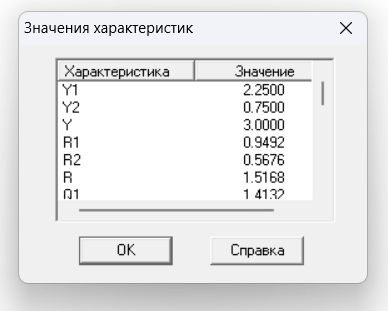
\includegraphics[width=.43\linewidth,height=5.6cm,keepaspectratio]{evidence/system1_R.png} &
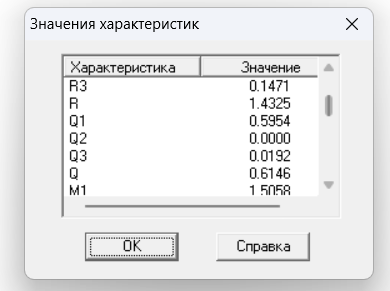
\includegraphics[width=.43\linewidth,height=5.6cm,keepaspectratio]{evidence/system2_R.png}\\[5pt]
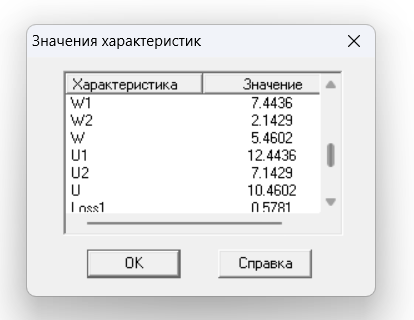
\includegraphics[width=.43\linewidth,height=5.6cm,keepaspectratio]{evidence/system1_times.png} &
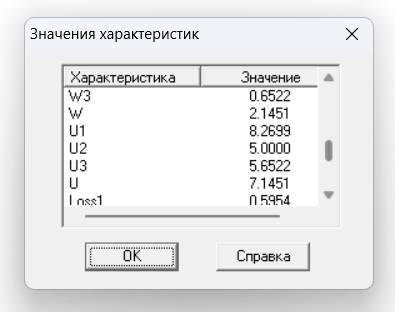
\includegraphics[width=.43\linewidth,height=5.6cm,keepaspectratio]{evidence/system2_times.png}\\[5pt]
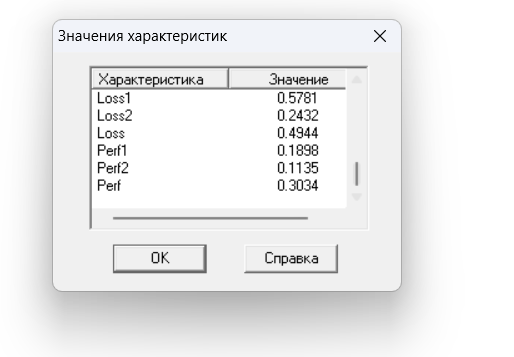
\includegraphics[width=.43\linewidth,height=5.6cm,keepaspectratio]{evidence/system1_output.png} &
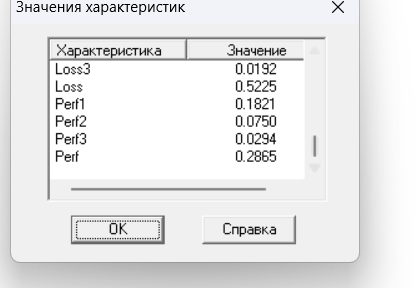
\includegraphics[width=.43\linewidth,height=5.6cm,keepaspectratio]{evidence/system2_output.png}
\end{tabular}
\caption{Результаты непосредственного расчёта в WinMark при исходной нагрузке. Снимки содержат значения $R$, $W$, $U$, \texttt{Loss} и \texttt{Perf}.}\label{fig:markwindows}
\end{figure}

\clearpage
\subsection{Параметры варьирования и экспорт графиков}
В окне «Данные $\to$ Варьируемые элементы» заданы 40 точек. Начальное значение и шаг каждого входного элемента одинаковы; \texttt{mu} и \texttt{nu} не варьируются. Параметры приведены в таблице~\ref{tab:markvary} и на рисунке~\ref{fig:markvary}.
\begin{table}[H]\centering\small
\caption{Варьирование интенсивностей в WinMark}\label{tab:markvary}
\begin{tabular}{@{}clrr@{}}\toprule
Система & Элемент & Начальное значение & Шаг\\\midrule
1 & \texttt{l1} & $0{,}0375$ & $0{,}0375$\\
1 & \texttt{l2} & $0{,}0125$ & $0{,}0125$\\
1 & \texttt{mu} & $0{,}2000$ & $0$\\\addlinespace
2 & \texttt{l1} & $0{,}0375$ & $0{,}0375$\\
2 & \texttt{l2} & $0{,}0100$ & $0{,}0100$\\
2 & \texttt{l3} & $0{,}0025$ & $0{,}0025$\\
2 & \texttt{mu} & $0{,}2000$ & $0$\\
2 & \texttt{nu} & $0{,}4000$ & $0$\\\bottomrule
\end{tabular}
\end{table}
\begin{figure}[H]\centering
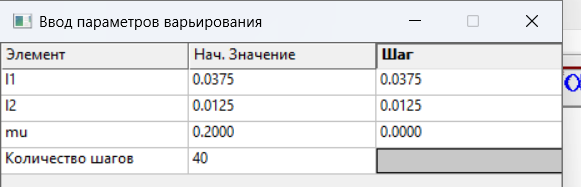
\includegraphics[width=.47\linewidth]{evidence/system1_variation.png}\hfill
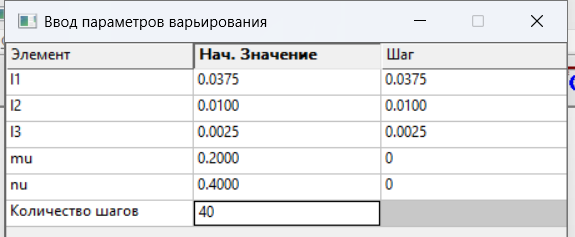
\includegraphics[width=.47\linewidth]{evidence/system2_variation.png}
\caption{Окна ввода параметров варьирования: слева \sysone, справа \systwo.}\label{fig:markvary}
\end{figure}

Для шага $h=1,\ldots,40$ общая интенсивность равна $\lambda_h=0{,}05h\secunit$. Шаг~12 соответствует $\lambda=0{,}6\secunit$. На графиках, экспортированных самой программой, абсцисса является индексом $j=h-1$ (от 0 до 39), поэтому $\lambda=0{,}05(j+1)\secunit$. На сравнительных графиках следующего раздела абсциссы переведены в физические значения $\lambda$.

Для каждой системы экспортированы шесть отдельных графиков: \texttt{R}, \texttt{Loss}, \texttt{Perf}, \texttt{Q}, \texttt{W}, \texttt{U}. Рисунок~\ref{fig:markR} показывает исходные графики критерия выбора; все 12 изображений входят в электронное приложение. Перед экспортом характеристик в точке восстановлены исходные элементы и повторно выполнены команды расчёта вероятностей и формул. Поэтому значения в точке в обоих HTML-отчётах относятся к $\lambda=0{,}6\secunit$.

\paragraph{Электронное приложение.}
В папке \texttt{docs} вместе с исходником отчёта находятся \path{system1/report_system1.html}, \path{system2/report_system2.html}, папки с графиками и использованные снимки окон. Сохранённые модели обеих систем находятся в \path{../WinMark/out/system1_33.mrk} и \path{../WinMark/out/system2_73.mrk}. В HTML ссылки на изображения заменены относительными и явно указана исходная кодировка Windows-1251, чтобы отчёты открывались после переноса папки. Числа, матрицы и формулы оставлены без изменений.

\clearpage
\begin{figure}[H]\centering
\textbf{\sysone}\\[3pt]
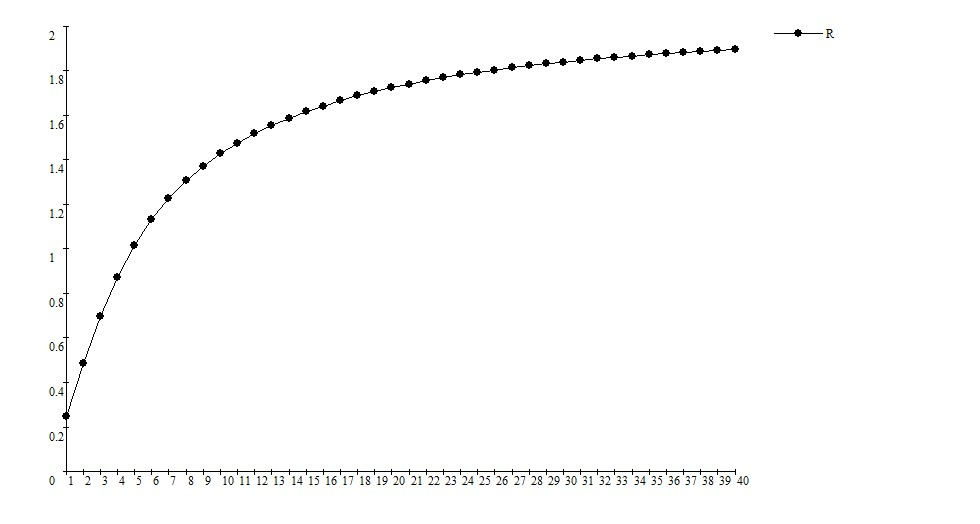
\includegraphics[width=.86\linewidth]{system1/graphics_system1/system1_R.JPG}\\[10pt]
\textbf{\systwo}\\[3pt]
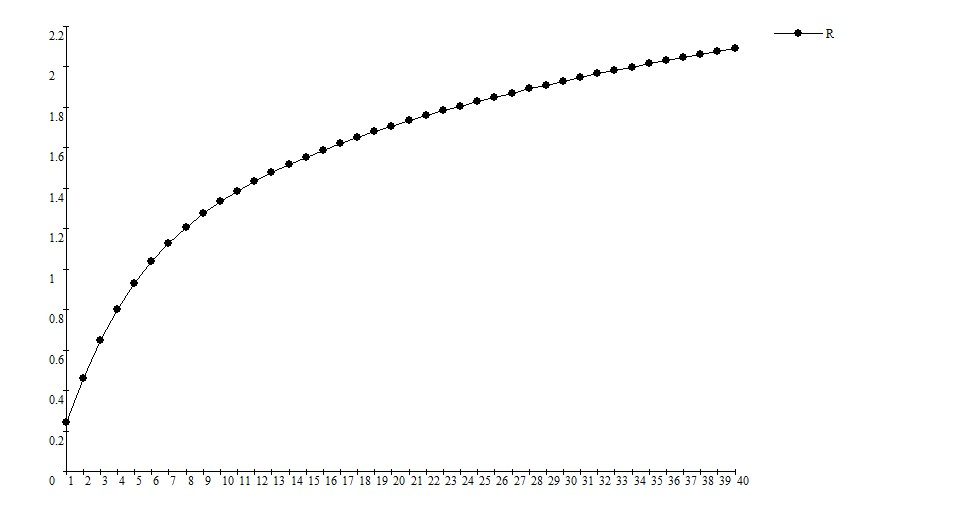
\includegraphics[width=.86\linewidth]{system2/graphics_system2/system2_R.JPG}
\caption{Графики загрузки $R$, непосредственно экспортированные из WinMark. По горизонтали показан индекс точки $j$; соответствующая интенсивность равна $0{,}05(j+1)\secunit$.}\label{fig:markR}
\end{figure}

\clearpage
\section{Сравнительный анализ систем}
\subsection{Варьирование интенсивности входного потока}
Интенсивность изменяется от $0{,}05$ до $2{,}00\secunit$ с шагом $0{,}05$ (40 точек), а $q_i$, $b$, законы обслуживания и накопители сохраняются. В каждой точке WinMark рассчитывает вероятности и все характеристики; результаты независимо проверяются на Python. Кривые ниже построены по числам из HTML-экспорта WinMark. Вертикальная пунктирная линия на графиках показывает исходное значение $\lambda=0{,}6\secunit$.

\begin{table}[H]\centering\small
\caption{Результаты в опорных точках варьирования}
\setlength{\tabcolsep}{6pt}
\begin{tabular}{@{}r rrrrrr@{}}\toprule
&\multicolumn{2}{c}{Загрузка $R$}&\multicolumn{2}{c}{Потери $\pi$}&\multicolumn{2}{c}{Пребывание $U$, с}\\
$\lambda$, $\text{с}^{-1}$ & СИСТ.1 & СИСТ.2 & СИСТ.1 & СИСТ.2 & СИСТ.1 & СИСТ.2\\\midrule
$0{,}20$ & $0{,}8724$ & $0{,}8030$ & $0{,}1276$ & $0{,}1970$ & $8{,}2205$ & $6{,}3728$ \\
$0{,}40$ & $1{,}3055$ & $1{,}2060$ & $0{,}3473$ & $0{,}3970$ & $9{,}7896$ & $6{,}9134$ \\
$0{,}60$ & $1{,}5168$ & $1{,}4325$ & $0{,}4944$ & $0{,}5225$ & $10{,}4602$ & $7{,}1451$ \\
$1{,}00$ & $1{,}7237$ & $1{,}7068$ & $0{,}6553$ & $0{,}6586$ & $11{,}0349$ & $7{,}3121$ \\
$1{,}50$ & $1{,}8389$ & $1{,}9281$ & $0{,}7548$ & $0{,}7429$ & $11{,}3694$ & $7{,}3784$ \\
$2{,}00$ & $1{,}8954$ & $2{,}0894$ & $0{,}8105$ & $0{,}7911$ & $11{,}5699$ & $7{,}4177$ \\
\bottomrule\end{tabular}
\end{table}

При исходной нагрузке первая система имеет большую суммарную загрузку, меньшие потери и большую производительность. При увеличении $\lambda$ преимущество по $R$ меняется: уточнение на Python между точками варьирования, то есть численное решение уравнения $R^{(1)}(\lambda)=R^{(2)}(\lambda)$, даёт
\[
\lambda_*\approx1{,}083188\secunit.
\]
На исследованном диапазоне первая система лучше по $R$ при $\lambda<\lambda_*$, вторая --- при $\lambda>\lambda_*$. При одинаковом $b$ в обоих вариантах $R=bX$, поэтому пересечение производительностей происходит в той же точке. Для положительной общей интенсивности пересечение потерь также совпадает с ней. Вывод о победителе относится прежде всего к заданной нагрузке $\lambda=0{,}6$, а не ко всем возможным нагрузкам.

\clearpage
\begin{figure}[H]\centering
\begin{tikzpicture}
\begin{axis}[width=.94\linewidth,height=6.6cm,
xlabel={$\lambda$, $\text{с}^{-1}$},ylabel={$R$, приборов},
xmin=0,xmax=2,grid=both,minor tick num=1,
legend style={font=\small,at={(.98,.03)},anchor=south east,draw=none,fill=white},
tick label style={font=\small},label style={font=\small},
/pgf/number format/use comma,title={Суммарная загрузка системы},title style={font=\small}]
\addplot[blue!70!black,thick] coordinates {(0.05,0.2487660000) (0.10,0.4856790000) (0.15,0.6959370000) (0.20,0.8723810000) (0.25,1.0161620000) (0.30,1.1324980000) (0.35,1.2272640000) (0.40,1.3054950000) (0.45,1.3710690000) (0.50,1.4268490000) (0.55,1.4749200000) (0.60,1.5168140000) (0.65,1.5536670000) (0.70,1.5863410000) (0.75,1.6155000000) (0.80,1.6416670000) (0.85,1.6652600000) (0.90,1.6866220000) (0.95,1.7060330000) (1.00,1.7237280000) (1.05,1.7399070000) (1.10,1.7547370000) (1.15,1.7683660000) (1.20,1.7809180000) (1.25,1.7925020000) (1.30,1.8032160000) (1.35,1.8131420000) (1.40,1.8223550000) (1.45,1.8309210000) (1.50,1.8388960000) (1.55,1.8463350000) (1.60,1.8532820000) (1.65,1.8597790000) (1.70,1.8658640000) (1.75,1.8715710000) (1.80,1.8769280000) (1.85,1.8819640000) (1.90,1.8867040000) (1.95,1.8911690000) (2.00,1.8953810000)};
\addlegendentry{СИСТЕМА\_1}
\addplot[red!75!black,thick,dashed] coordinates {(0.05,0.2433260000) (0.10,0.4617900000) (0.15,0.6479710000) (0.20,0.8029780000) (0.25,0.9314080000) (0.30,1.0384690000) (0.35,1.1287750000) (0.40,1.2060430000) (0.45,1.2731340000) (0.50,1.3322210000) (0.55,1.3849360000) (0.60,1.4325170000) (0.65,1.4759040000) (0.70,1.5158200000) (0.75,1.5528250000) (0.80,1.5873600000) (0.85,1.6197740000) (0.90,1.6503480000) (0.95,1.6793080000) (1.00,1.7068410000) (1.05,1.7331010000) (1.10,1.7582150000) (1.15,1.7822920000) (1.20,1.8054250000) (1.25,1.8276910000) (1.30,1.8491590000) (1.35,1.8698870000) (1.40,1.8899280000) (1.45,1.9093270000) (1.50,1.9281230000) (1.55,1.9463530000) (1.60,1.9640500000) (1.65,1.9812410000) (1.70,1.9979530000) (1.75,2.0142100000) (1.80,2.0300330000) (1.85,2.0454420000) (1.90,2.0604560000) (1.95,2.0750910000) (2.00,2.0893630000)};
\addlegendentry{СИСТЕМА\_2}
\draw[densely dotted,gray] (axis cs:.6,\pgfkeysvalueof{/pgfplots/ymin}) -- (axis cs:.6,\pgfkeysvalueof{/pgfplots/ymax});
\end{axis}
\end{tikzpicture}
\vspace{.5cm}
\begin{tikzpicture}
\begin{axis}[width=.94\linewidth,height=6.6cm,
xlabel={$\lambda$, $\text{с}^{-1}$},ylabel={$\pi$},
xmin=0,xmax=2,grid=both,minor tick num=1,
legend style={font=\small,at={(.98,.03)},anchor=south east,draw=none,fill=white},
tick label style={font=\small},label style={font=\small},
/pgf/number format/use comma,title={Вероятность потери заявки},title style={font=\small}]
\addplot[blue!70!black,thick] coordinates {(0.05,0.0049380000) (0.10,0.0286430000) (0.15,0.0720850000) (0.20,0.1276190000) (0.25,0.1870700000) (0.30,0.2450010000) (0.35,0.2987060000) (0.40,0.3472530000) (0.45,0.3906360000) (0.50,0.4292610000) (0.55,0.4636650000) (0.60,0.4943950000) (0.65,0.5219480000) (0.70,0.5467600000) (0.75,0.5692000000) (0.80,0.5895830000) (0.85,0.6081740000) (0.90,0.6251950000) (0.95,0.6408350000) (1.00,0.6552540000) (1.05,0.6685890000) (1.10,0.6809570000) (1.15,0.6924580000) (1.20,0.7031800000) (1.25,0.7132000000) (1.30,0.7225820000) (1.35,0.7313860000) (1.40,0.7396640000) (1.45,0.7474590000) (1.50,0.7548140000) (1.55,0.7617630000) (1.60,0.7683400000) (1.65,0.7745720000) (1.70,0.7804870000) (1.75,0.7861060000) (1.80,0.7914520000) (1.85,0.7965440000) (1.90,0.8014000000) (1.95,0.8060340000) (2.00,0.8104620000)};
\addlegendentry{СИСТЕМА\_1}
\addplot[red!75!black,thick,dashed] coordinates {(0.05,0.0266930000) (0.10,0.0764210000) (0.15,0.1360380000) (0.20,0.1970220000) (0.25,0.2548730000) (0.30,0.3076870000) (0.35,0.3549850000) (0.40,0.3969790000) (0.45,0.4341620000) (0.50,0.4671120000) (0.55,0.4963870000) (0.60,0.5224940000) (0.65,0.5458760000) (0.70,0.5669090000) (0.75,0.5859130000) (0.80,0.6031600000) (0.85,0.6188770000) (0.90,0.6332560000) (0.95,0.6464610000) (1.00,0.6586320000) (1.05,0.6698860000) (1.10,0.6803250000) (1.15,0.6900360000) (1.20,0.6990960000) (1.25,0.7075700000) (1.30,0.7155140000) (1.35,0.7229800000) (1.40,0.7300100000) (1.45,0.7366450000) (1.50,0.7429170000) (1.55,0.7488580000) (1.60,0.7544940000) (1.65,0.7598490000) (1.70,0.7649470000) (1.75,0.7698050000) (1.80,0.7744410000) (1.85,0.7788710000) (1.90,0.7831100000) (1.95,0.7871700000) (2.00,0.7910640000)};
\addlegendentry{СИСТЕМА\_2}
\draw[densely dotted,gray] (axis cs:.6,\pgfkeysvalueof{/pgfplots/ymin}) -- (axis cs:.6,\pgfkeysvalueof{/pgfplots/ymax});
\end{axis}
\end{tikzpicture}
\caption{Влияние входной интенсивности на суммарную загрузку и вероятность потери.}\label{fig:rpi}
\end{figure}

\clearpage
\begin{figure}[H]\centering
\begin{tikzpicture}
\begin{axis}[width=.94\linewidth,height=6.6cm,
xlabel={$\lambda$, $\text{с}^{-1}$},ylabel={$X$, $\text{с}^{-1}$},
xmin=0,xmax=2,grid=both,minor tick num=1,
legend style={font=\small,at={(.98,.03)},anchor=south east,draw=none,fill=white},
tick label style={font=\small},label style={font=\small},
/pgf/number format/use comma,title={Производительность системы},title style={font=\small}]
\addplot[blue!70!black,thick] coordinates {(0.05,0.0497530000) (0.10,0.0971360000) (0.15,0.1391870000) (0.20,0.1744760000) (0.25,0.2032320000) (0.30,0.2265000000) (0.35,0.2454530000) (0.40,0.2610990000) (0.45,0.2742140000) (0.50,0.2853700000) (0.55,0.2949840000) (0.60,0.3033630000) (0.65,0.3107330000) (0.70,0.3172680000) (0.75,0.3231000000) (0.80,0.3283330000) (0.85,0.3330520000) (0.90,0.3373240000) (0.95,0.3412070000) (1.00,0.3447460000) (1.05,0.3479810000) (1.10,0.3509470000) (1.15,0.3536730000) (1.20,0.3561840000) (1.25,0.3585000000) (1.30,0.3606430000) (1.35,0.3626280000) (1.40,0.3644710000) (1.45,0.3661840000) (1.50,0.3677790000) (1.55,0.3692670000) (1.60,0.3706560000) (1.65,0.3719560000) (1.70,0.3731730000) (1.75,0.3743140000) (1.80,0.3753860000) (1.85,0.3763930000) (1.90,0.3773410000) (1.95,0.3782340000) (2.00,0.3790760000)};
\addlegendentry{СИСТЕМА\_1}
\addplot[red!75!black,thick,dashed] coordinates {(0.05,0.0486650000) (0.10,0.0923580000) (0.15,0.1295940000) (0.20,0.1605960000) (0.25,0.1862820000) (0.30,0.2076940000) (0.35,0.2257550000) (0.40,0.2412090000) (0.45,0.2546270000) (0.50,0.2664440000) (0.55,0.2769870000) (0.60,0.2865030000) (0.65,0.2951810000) (0.70,0.3031640000) (0.75,0.3105650000) (0.80,0.3174720000) (0.85,0.3239550000) (0.90,0.3300700000) (0.95,0.3358620000) (1.00,0.3413680000) (1.05,0.3466200000) (1.10,0.3516430000) (1.15,0.3564590000) (1.20,0.3610850000) (1.25,0.3655380000) (1.30,0.3698320000) (1.35,0.3739780000) (1.40,0.3779860000) (1.45,0.3818650000) (1.50,0.3856250000) (1.55,0.3892710000) (1.60,0.3928100000) (1.65,0.3962480000) (1.70,0.3995910000) (1.75,0.4028420000) (1.80,0.4060070000) (1.85,0.4090880000) (1.90,0.4120910000) (1.95,0.4150180000) (2.00,0.4178730000)};
\addlegendentry{СИСТЕМА\_2}
\draw[densely dotted,gray] (axis cs:.6,\pgfkeysvalueof{/pgfplots/ymin}) -- (axis cs:.6,\pgfkeysvalueof{/pgfplots/ymax});
\end{axis}
\end{tikzpicture}
\vspace{.5cm}
\begin{tikzpicture}
\begin{axis}[width=.94\linewidth,height=6.6cm,
xlabel={$\lambda$, $\text{с}^{-1}$},ylabel={$L$, заявок},
xmin=0,xmax=2,grid=both,minor tick num=1,
legend style={font=\small,at={(.98,.03)},anchor=south east,draw=none,fill=white},
tick label style={font=\small},label style={font=\small},
/pgf/number format/use comma,title={Суммарная средняя длина очередей},title style={font=\small}]
\addplot[blue!70!black,thick] coordinates {(0.05,0.0429880000) (0.10,0.1706100000) (0.15,0.3556380000) (0.20,0.5619050000) (0.25,0.7633700000) (0.30,0.9471440000) (0.35,1.1093240000) (0.40,1.2505490000) (0.45,1.3732160000) (0.50,1.4800930000) (0.55,1.5737570000) (0.60,1.6564070000) (0.65,1.7298560000) (0.70,1.7955740000) (0.75,1.8547460000) (0.80,1.9083330000) (0.85,1.9571160000) (0.90,2.0017350000) (0.95,2.0427180000) (1.00,2.0805060000) (1.05,2.1154690000) (1.10,2.1479180000) (1.15,2.1781200000) (1.20,2.2063050000) (1.25,2.2326700000) (1.30,2.2573870000) (1.35,2.2806070000) (1.40,2.3024620000) (1.45,2.3230680000) (1.50,2.3425300000) (1.55,2.3609390000) (1.60,2.3783780000) (1.65,2.3949210000) (1.70,2.4106350000) (1.75,2.4255800000) (1.80,2.4398080000) (1.85,2.4533720000) (1.90,2.4663150000) (1.95,2.4786780000) (2.00,2.4904990000)};
\addlegendentry{СИСТЕМА\_1}
\addplot[red!75!black,thick,dashed] coordinates {(0.05,0.0230370000) (0.10,0.0782200000) (0.15,0.1478650000) (0.20,0.2204690000) (0.25,0.2899170000) (0.30,0.3535700000) (0.35,0.4107030000) (0.40,0.4615230000) (0.45,0.5066230000) (0.50,0.5467120000) (0.55,0.5824850000) (0.60,0.6145690000) (0.65,0.6435140000) (0.70,0.6697830000) (0.75,0.6937690000) (0.80,0.7158020000) (0.85,0.7361580000) (0.90,0.7550660000) (0.95,0.7727220000) (1.00,0.7892870000) (1.05,0.8049000000) (1.10,0.8196770000) (1.15,0.8337170000) (1.20,0.8471050000) (1.25,0.8599130000) (1.30,0.8722040000) (1.35,0.8840290000) (1.40,0.8954370000) (1.45,0.9064670000) (1.50,0.9171540000) (1.55,0.9275280000) (1.60,0.9376160000) (1.65,0.9474400000) (1.70,0.9570230000) (1.75,0.9663810000) (1.80,0.9755310000) (1.85,0.9844870000) (1.90,0.9932610000) (1.95,1.0018640000) (2.00,1.0103070000)};
\addlegendentry{СИСТЕМА\_2}
\draw[densely dotted,gray] (axis cs:.6,\pgfkeysvalueof{/pgfplots/ymin}) -- (axis cs:.6,\pgfkeysvalueof{/pgfplots/ymax});
\end{axis}
\end{tikzpicture}
\caption{Производительность и суммарная средняя длина очередей при варьировании $\lambda$.}\label{fig:xl}
\end{figure}

\clearpage
\begin{figure}[H]\centering
\begin{tikzpicture}
\begin{axis}[width=.94\linewidth,height=6.6cm,
xlabel={$\lambda$, $\text{с}^{-1}$},ylabel={$W$, с},
xmin=0,xmax=2,grid=both,minor tick num=1,
legend style={font=\small,at={(.98,.03)},anchor=south east,draw=none,fill=white},
tick label style={font=\small},label style={font=\small},
/pgf/number format/use comma,title={Среднее ожидание принятой заявки},title style={font=\small}]
\addplot[blue!70!black,thick] coordinates {(0.05,0.8640210000) (0.10,1.7564110000) (0.15,2.5551060000) (0.20,3.2205250000) (0.25,3.7561450000) (0.30,4.1816590000) (0.35,4.5195020000) (0.40,4.7895620000) (0.45,5.0078270000) (0.50,5.1865810000) (0.55,5.3350550000) (0.60,5.4601530000) (0.65,5.5670100000) (0.70,5.6594830000) (0.75,5.7404720000) (0.80,5.8121830000) (0.85,5.8763060000) (0.90,5.9341550000) (0.95,5.9867500000) (1.00,6.0349040000) (1.05,6.0792620000) (1.10,6.1203390000) (1.15,6.1585700000) (1.20,6.1942920000) (1.25,6.2278000000) (1.30,6.2593350000) (1.35,6.2891020000) (1.40,6.3172700000) (1.45,6.3439910000) (1.50,6.3693900000) (1.55,6.3935820000) (1.60,6.4166680000) (1.65,6.4387240000) (1.70,6.4598360000) (1.75,6.4800650000) (1.80,6.4994720000) (1.85,6.5181130000) (1.90,6.5360420000) (1.95,6.5532970000) (2.00,6.5699180000)};
\addlegendentry{СИСТЕМА\_1}
\addplot[red!75!black,thick,dashed] coordinates {(0.05,0.4733720000) (0.10,0.8469260000) (0.15,1.1409800000) (0.20,1.3728210000) (0.25,1.5563360000) (0.30,1.7023610000) (0.35,1.8192420000) (0.40,1.9133770000) (0.45,1.9896690000) (0.50,2.0518830000) (0.55,2.1029300000) (0.60,2.1450690000) (0.65,2.1800660000) (0.70,2.2093100000) (0.75,2.2338940000) (0.80,2.2546940000) (0.85,2.2724090000) (0.90,2.2875970000) (0.95,2.3007130000) (1.00,2.3121260000) (1.05,2.3221380000) (1.10,2.3309910000) (1.15,2.3388900000) (1.20,2.3460000000) (1.25,2.3524580000) (1.30,2.3583800000) (1.35,2.3638580000) (1.40,2.3689710000) (1.45,2.3737880000) (1.50,2.3783590000) (1.55,2.3827310000) (1.60,2.3869430000) (1.65,2.3910270000) (1.70,2.3950090000) (1.75,2.3989110000) (1.80,2.4027470000) (1.85,2.4065410000) (1.90,2.4102940000) (1.95,2.4140240000) (2.00,2.4177390000)};
\addlegendentry{СИСТЕМА\_2}
\draw[densely dotted,gray] (axis cs:.6,\pgfkeysvalueof{/pgfplots/ymin}) -- (axis cs:.6,\pgfkeysvalueof{/pgfplots/ymax});
\end{axis}
\end{tikzpicture}
\vspace{.5cm}
\begin{tikzpicture}
\begin{axis}[width=.94\linewidth,height=6.6cm,
xlabel={$\lambda$, $\text{с}^{-1}$},ylabel={$U$, с},
xmin=0,xmax=2,grid=both,minor tick num=1,
legend style={font=\small,at={(.98,.03)},anchor=south east,draw=none,fill=white},
tick label style={font=\small},label style={font=\small},
/pgf/number format/use comma,title={Среднее пребывание принятой заявки},title style={font=\small}]
\addplot[blue!70!black,thick] coordinates {(0.05,5.8640200000) (0.10,6.7564110000) (0.15,7.5551060000) (0.20,8.2205260000) (0.25,8.7561450000) (0.30,9.1816580000) (0.35,9.5195020000) (0.40,9.7895610000) (0.45,10.0078260000) (0.50,10.1865810000) (0.55,10.3350540000) (0.60,10.4601530000) (0.65,10.5670090000) (0.70,10.6594840000) (0.75,10.7404710000) (0.80,10.8121830000) (0.85,10.8763050000) (0.90,10.9341550000) (0.95,10.9867490000) (1.00,11.0349030000) (1.05,11.0792630000) (1.10,11.1203390000) (1.15,11.1585710000) (1.20,11.1942920000) (1.25,11.2278000000) (1.30,11.2593350000) (1.35,11.2891040000) (1.40,11.3172700000) (1.45,11.3439910000) (1.50,11.3693900000) (1.55,11.3935800000) (1.60,11.4166670000) (1.65,11.4387220000) (1.70,11.4598370000) (1.75,11.4800650000) (1.80,11.4994710000) (1.85,11.5181110000) (1.90,11.5360420000) (1.95,11.5532980000) (2.00,11.5699180000)};
\addlegendentry{СИСТЕМА\_1}
\addplot[red!75!black,thick,dashed] coordinates {(0.05,5.4733720000) (0.10,5.8469260000) (0.15,6.1409800000) (0.20,6.3728210000) (0.25,6.5563360000) (0.30,6.7023600000) (0.35,6.8192420000) (0.40,6.9133760000) (0.45,6.9896700000) (0.50,7.0518830000) (0.55,7.1029310000) (0.60,7.1450700000) (0.65,7.1800660000) (0.70,7.2093110000) (0.75,7.2338950000) (0.80,7.2546940000) (0.85,7.2724100000) (0.90,7.2875970000) (0.95,7.3007140000) (1.00,7.3121250000) (1.05,7.3221390000) (1.10,7.3309930000) (1.15,7.3388920000) (1.20,7.3460020000) (1.25,7.3524590000) (1.30,7.3583820000) (1.35,7.3638600000) (1.40,7.3689700000) (1.45,7.3737880000) (1.50,7.3783590000) (1.55,7.3827290000) (1.60,7.3869400000) (1.65,7.3910250000) (1.70,7.3950080000) (1.75,7.3989110000) (1.80,7.4027470000) (1.85,7.4065450000) (1.90,7.4102940000) (1.95,7.4140240000) (2.00,7.4177380000)};
\addlegendentry{СИСТЕМА\_2}
\draw[densely dotted,gray] (axis cs:.6,\pgfkeysvalueof{/pgfplots/ymin}) -- (axis cs:.6,\pgfkeysvalueof{/pgfplots/ymax});
\end{axis}
\end{tikzpicture}
\caption{Времена ожидания и пребывания принятых заявок, рассчитанные прямым усреднением по состояниям.}\label{fig:wu}
\end{figure}

\subsection{Объяснение различий и влияние накопителей}
Обе системы направляют $75\%$ входного потока к П1: его предлагаемая нагрузка $y_1=2{,}25$ существенно больше единицы. Во второй системе третий прибор получает лишь $5\%$ потока; свободная мощность П2 и П3 не может обслужить заявки, потерянные у П1. Поэтому большее число приборов само по себе не обеспечивает большую суммарную загрузку при заданном правиле направления.

Преимущество первой системы при исходном $\lambda$ связано с большим накопителем перед перегруженным П1 и наличием накопителя перед П2. У первой системы П2 принимает $25\%$ потока и имеет одно место ожидания; у второй --- только $20\%$ и работает без накопителя. Это более чем компенсирует наличие малозагруженного П3 во второй системе.

Влияние ёмкости нельзя оценивать путём прямого сравнения разных законов обслуживания и разного числа приборов. Для отдельной проверки рассмотрен \emph{один и тот же} экспоненциальный П1 с $\lambda_1=0{,}45\secunit$, $b=5$ с и разным числом мест ожидания:

\begin{table}[H]\centering\small
\caption{Контроль влияния накопителя при неизменных остальных параметрах}
\begin{tabular}{@{}crrr@{}}\toprule
Места ожидания & Потери $\pi_1$ & Загрузка $\rho_1$ & Ожидание $w_1$, с\\\midrule
0 & $0{,}692308$ & $0{,}692308$ & $0{,}000000$ \\
1 & $0{,}609023$ & $0{,}879699$ & $3{,}461538$ \\
2 & $0{,}578113$ & $0{,}949247$ & $7{,}443609$ \\
\bottomrule\end{tabular}
\end{table}

Увеличение накопителя в данном контроле \textbf{уменьшает потери и повышает загрузку}, одновременно увеличивая среднее ожидание принятых заявок. Поэтому вывод о том, что накопитель только увеличивает ожидание и не снижает потери, для рассматриваемых моделей неверен.

Чтобы отделить эффект распределения обслуживания, сравним при \emph{одном месте ожидания} экспоненциальный и эрланговский П1. Замена экспоненциального обслуживания на $E_2$ с тем же средним снижает потери с $0{,}609023$ до $0{,}595380$, повышает загрузку с $0{,}879699$ до $0{,}910396$ и уменьшает ожидание с $3{,}461538$ до $3{,}269896$ с. Этот выигрыш второй системы не устраняет преимущество первой по суммарной загрузке при исходной интенсивности.


\subsection{Влияние выбора прибора с обслуживанием \texorpdfstring{$E_2$}{E2}}\label{sec:placement}
В соответствии с заданием закон Эрланга назначается ровно одному прибору, причём его можно выбрать. В основной модели выбран П1. Чтобы проверить зависимость вывода от этого решения, дополнительно рассчитаны все три допустимых размещения $E_2$ при исходной интенсивности. Этот контроль выполнен программой на Python (функция \texttt{placement\_study}); основной расчёт WinMark и его графики относятся только к $E_2$ в П1.

Во всех трёх случаях сохранены накопители $1/0/1$, вероятности направления $(0{,}75;0{,}20;0{,}05)$ и среднее обслуживание $b=5$ с. Меняется только прибор с двумя последовательными фазами. Если выбран П1 или П3, число состояний равно $5\cdot2\cdot3=30$ или $3\cdot2\cdot5=30$. Если выбран П2 без накопителя, его локальные состояния --- свободен, первая фаза, вторая фаза; полная модель содержит $3\cdot3\cdot3=27$ состояний.

\begin{table}[H]\centering\small
\caption{Контроль размещения $E_2$ во второй системе при $\lambda=0{,}6\secunit$}\label{tab:placement}
\begin{tabular}{@{}ccrrr@{}}\toprule
Прибор с $E_2$ & Состояний & Загрузка $R$ & Производительность $X$ & Потери $\pi$\\\midrule
П1 & 30 & $1{,}432517$ & $0{,}286503$ & $0{,}522494$ \\
П2 & 27 & $1{,}401821$ & $0{,}280364$ & $0{,}532726$ \\
П3 & 30 & $1{,}402434$ & $0{,}280487$ & $0{,}532522$ \\
\bottomrule\end{tabular}
\end{table}

Прибор П2 не имеет очереди. При сохранении среднего обслуживания его вероятность занятости равна $\lambda_2b/(1+\lambda_2b)=0{,}375$ как для экспоненциального, так и для эрланговского закона; принятое поступление начинает обслуживание сразу. Поэтому перенос $E_2$ в П2 не даёт выигрыша от уменьшения разброса времени обслуживания в очереди.

Среди трёх размещений наибольшая суммарная загрузка второй системы достигается при $E_2$ в П1: $R=1{,}432517$. Но и она меньше $R^{(1)}=1{,}516814$. Следовательно, \textbf{при исходной нагрузке выбор первой системы сохраняется при любом допустимом выборе прибора с $E_2$}. Положение точки пересечения при варьировании, найденное выше, относится именно к основному размещению $E_2$ в П1.

\section{Выбор наилучшего варианта организации системы}
По заданному критерию максимальной загрузки при $\lambda=0{,}6\secunit$ выбирается \textbf{\sysone}:
\[
R^{(1)}=1{,}516814>R^{(2)}=1{,}432517.
\]
Абсолютный выигрыш составляет $0{,}084297$ одновременно работающего прибора в среднем, относительный --- $5{,}88\%$ относительно второй системы. Контроль размещения $E_2$ подтвердил этот выбор для всех трёх допустимых приборов второй системы (таблица~\ref{tab:placement}). Средняя загрузка одного прибора также выше: $0{,}758407>0{,}477506$, поэтому выбор при исходных данных одинаков для суммарного и нормированного показателей.

Первая система обслуживает $0{,}303363$ заявки в секунду против $0{,}286503$; потери ниже на $2{,}809905$ процентного пункта ($49{,}44\%$ против $52{,}25\%$). При этом она имеет более длинные очереди и большее время пребывания: $10{,}460153$ с против $7{,}145069$ с. Следовательно, вторая система лучше по временным показателям, однако эти показатели не являются критерием данного варианта.

\section{Выводы}
Построены полные марковские модели варианта 33/73/11: двухприборная \sysone\ с накопителями $2/1$ и трёхприборная \systwo\ с накопителями $1/0/1$, в которой только П1 имеет обслуживание Эрланга второго порядка. Получены размеченные графы, генераторы размером $12\times12$ и $30\times30$, стационарные вероятности и все характеристики формы~2.

Расчёты выполнены в WinMark и подтверждены снимками окон, полными HTML-отчётами и экспортированными графиками. Независимая программа на Python проверила все 40 точек варьирования: 2240 значений характеристик и 1680 вероятностей; максимальное расхождение с WinMark меньше $10^{-5}$. Времена ожидания и пребывания определены через распределение состояний в момент поступления принятой заявки и остаточное число фаз обслуживания. Формулы Литтла применены после расчёта для проверки. Стационарные вероятности дополнительно сверены с независимым аналитическим решением для отдельных приборов; максимальные расхождения находятся на уровне машинной точности.

При заданном $\lambda=0{,}6\secunit$ лучшей по максимальной суммарной загрузке является \sysone\ ($R=1{,}516814$ против $1{,}432517$), хотя \systwo\ обеспечивает меньшее время пребывания. В диапазоне варьирования победитель по суммарной загрузке меняется около $\lambda=1{,}083188\secunit$. Дополнительная проверка всех трёх допустимых размещений $E_2$ сохранила выбор первой системы при исходной нагрузке. Контрольный расчёт при неизменных остальных параметрах подтвердил, что накопитель способен снижать потери и повышать загрузку ценой дополнительного ожидания.

\clearpage
\renewcommand{\refname}{Список использованных материалов}
\begin{thebibliography}{9}
\addcontentsline{toc}{section}{Список использованных материалов}
\bibitem{task} Учебно-исследовательская работа 2 (УИР 2). «Марковские модели систем массового обслуживания». Университет ИТМО, факультет ПИ и КТ. Задание от 23.09.2024. 7~с.
\bibitem{theory} Основы моделирования дискретных систем. Раздел~5 «Численное моделирование (модели случайных процессов)». Предоставленный теоретический материал «МП\_теория к УИР2». 68~с.
\bibitem{slides} Модели марковских случайных процессов (численное моделирование). Университет ИТМО, ФПИиКТ. Предоставленная презентация «ЧИСЛЕННОЕ МОДЕЛИРОВАНИЕ». 14~слайдов.
\bibitem{mark1} WinMark. Результаты расчёта \sysone\ (вариант 33), экспорт от 27.10.2026. Электронное приложение: \path{system1/report_system1.html}.
\bibitem{mark2} WinMark. Результаты расчёта \systwo\ (вариант 73), экспорт от 27.10.2026. Электронное приложение: \path{system2/report_system2.html}.
\end{thebibliography}

\appendix
\clearpage
\section{Полная численная матрица второй системы}\label{app:matrix}
Таблица задаёт все элементы $G_2$ при исходной нагрузке. В строке $i$ отдельно указан $g_{ii}$, затем пары $j:g_{ij}$ для \emph{всех} ненулевых внедиагональных элементов. Остальные элементы равны нулю. Это та же матрица, что в~\eqref{eq:q2}; порядок состояний соответствует таблице~\ref{tab:prob}.

{\small\renewcommand{\arraystretch}{1.08}
\begin{longtable}{@{}r r p{12.7cm}@{}}
\caption{Матрица $G_2$ в полном разреженном представлении}\\\toprule
$i$ & $g_{ii}$ & Ненулевые внедиагональные элементы $j:g_{ij}$, $\text{с}^{-1}$\\\midrule
\endfirsthead
\caption*{Таблица \thetable\ (продолжение)}\\\toprule
$i$ & $g_{ii}$ & Ненулевые внедиагональные элементы $j:g_{ij}$\\\midrule
\endhead\bottomrule\endfoot
0 & $-0{,}60$ & $1:0{,}03;\quad 3:0{,}12;\quad 6:0{,}45$ \\
1 & $-0{,}80$ & $0:0{,}20;\quad 2:0{,}03;\quad 4:0{,}12;\quad 7:0{,}45$ \\
2 & $-0{,}77$ & $1:0{,}20;\quad 5:0{,}12;\quad 8:0{,}45$ \\
3 & $-0{,}68$ & $0:0{,}20;\quad 4:0{,}03;\quad 9:0{,}45$ \\
4 & $-0{,}88$ & $1:0{,}20;\quad 3:0{,}20;\quad 5:0{,}03;\quad 10:0{,}45$ \\
5 & $-0{,}85$ & $2:0{,}20;\quad 4:0{,}20;\quad 11:0{,}45$ \\
6 & $-1{,}00$ & $7:0{,}03;\quad 9:0{,}12;\quad 12:0{,}40;\quad 18:0{,}45$ \\
7 & $-1{,}20$ & $6:0{,}20;\quad 8:0{,}03;\quad 10:0{,}12;\quad 13:0{,}40;\quad 19:0{,}45$ \\
8 & $-1{,}17$ & $7:0{,}20;\quad 11:0{,}12;\quad 14:0{,}40;\quad 20:0{,}45$ \\
9 & $-1{,}08$ & $6:0{,}20;\quad 10:0{,}03;\quad 15:0{,}40;\quad 21:0{,}45$ \\
10 & $-1{,}28$ & $7:0{,}20;\quad 9:0{,}20;\quad 11:0{,}03;\quad 16:0{,}40;\quad 22:0{,}45$ \\
11 & $-1{,}25$ & $8:0{,}20;\quad 10:0{,}20;\quad 17:0{,}40;\quad 23:0{,}45$ \\
12 & $-1{,}00$ & $0:0{,}40;\quad 13:0{,}03;\quad 15:0{,}12;\quad 24:0{,}45$ \\
13 & $-1{,}20$ & $1:0{,}40;\quad 12:0{,}20;\quad 14:0{,}03;\quad 16:0{,}12;\quad 25:0{,}45$ \\
14 & $-1{,}17$ & $2:0{,}40;\quad 13:0{,}20;\quad 17:0{,}12;\quad 26:0{,}45$ \\
15 & $-1{,}08$ & $3:0{,}40;\quad 12:0{,}20;\quad 16:0{,}03;\quad 27:0{,}45$ \\
16 & $-1{,}28$ & $4:0{,}40;\quad 13:0{,}20;\quad 15:0{,}20;\quad 17:0{,}03;\quad 28:0{,}45$ \\
17 & $-1{,}25$ & $5:0{,}40;\quad 14:0{,}20;\quad 16:0{,}20;\quad 29:0{,}45$ \\
18 & $-0{,}55$ & $19:0{,}03;\quad 21:0{,}12;\quad 24:0{,}40$ \\
19 & $-0{,}75$ & $18:0{,}20;\quad 20:0{,}03;\quad 22:0{,}12;\quad 25:0{,}40$ \\
20 & $-0{,}72$ & $19:0{,}20;\quad 23:0{,}12;\quad 26:0{,}40$ \\
21 & $-0{,}63$ & $18:0{,}20;\quad 22:0{,}03;\quad 27:0{,}40$ \\
22 & $-0{,}83$ & $19:0{,}20;\quad 21:0{,}20;\quad 23:0{,}03;\quad 28:0{,}40$ \\
23 & $-0{,}80$ & $20:0{,}20;\quad 22:0{,}20;\quad 29:0{,}40$ \\
24 & $-0{,}55$ & $6:0{,}40;\quad 25:0{,}03;\quad 27:0{,}12$ \\
25 & $-0{,}75$ & $7:0{,}40;\quad 24:0{,}20;\quad 26:0{,}03;\quad 28:0{,}12$ \\
26 & $-0{,}72$ & $8:0{,}40;\quad 25:0{,}20;\quad 29:0{,}12$ \\
27 & $-0{,}63$ & $9:0{,}40;\quad 24:0{,}20;\quad 28:0{,}03$ \\
28 & $-0{,}83$ & $10:0{,}40;\quad 25:0{,}20;\quad 27:0{,}20;\quad 29:0{,}03$ \\
29 & $-0{,}80$ & $11:0{,}40;\quad 26:0{,}20;\quad 28:0{,}20$ \\
\end{longtable}}

\clearpage
\section{Программа расчёта всех характеристик}\label{app:code}
Ниже приведён полный код независимого расчёта, использованный для проверки WinMark, построения таблиц и контрольных экспериментов. Требуется Python~3.10 или новее; сторонние библиотеки не нужны. Код хранится в \path{../app/calculate_uir2.py} и подключается к отчёту без создания копий. Для повторения вычислений из корня папки лабораторной работы нужно выполнить:
\begin{lstlisting}[language=bash,numbers=none]
python app/calculate_uir2.py
\end{lstlisting}
Программа выводит все вероятности, характеристики и опорные данные в консоль. Файлы \path{../out/results.json} и \path{../out/calculation_log.txt} автоматически сохраняются в папке \texttt{out} проекта независимо от рабочей папки запуска. Запуск Python требуется только для повторной проверки чисел. Для компиляции отчёта из папки \texttt{docs} нужно сохранить структуру проекта: снимки окон находятся в \texttt{evidence}, исходные графики --- в \texttt{system1/graphics\_system1} и \texttt{system2/graphics\_system2}, код --- в \texttt{../app}. Сравнительные кривые и численные таблицы встроены в \texttt{.tex}. Функции \texttt{metrics} и \texttt{calculate} показывают соответственно прямой расчёт показателей и последующую независимую проверку.

\lstinputlisting[basicstyle=\ttfamily\fontsize{8}{9}\selectfont,caption={Полный исходный код расчёта варианта 33/73/11}]{app/calculate_uir2.py}

\clearpage
\section{Протокол фактического выполнения}\label{app:log}
Ниже приведён фрагмент реального консольного вывода той же программы: заголовки запусков, все восемь характеристик каждого прибора и системы, максимальные невязки и контрольные расчёты. Полные вероятности и результаты варьирования из вывода перенесены в таблицы основной части отчёта; они также сохраняются программой в \texttt{results.json}.

\begin{lstlisting}[language={},numbers=none,basicstyle=\ttfamily\tiny]
Python 3.12.14
Variant 33/73/11; lambda=0.6; B=5; mu=0.2; nu=0.4

SYSTEM_1 states = 12
node      y        rho        l          m         pi         X          W          U
   1   2.250000   0.949247   1.413164   2.362411   0.578113   0.189849   7.443609  12.443609
   2   0.750000   0.567568   0.243243   0.810811   0.243243   0.113514   2.142857   7.142857
 ALL   3.000000   1.516814   1.656407   3.173222   0.494395   0.303363   5.460153  10.460153
max errors: rows=5.551e-17 stationary=4.510e-17 factorization=8.674e-17 all=1.776e-15

SYSTEM_2 states = 30
node      y        rho        l          m         pi         X          W          U
   1   2.250000   0.910396   0.595380   1.505775   0.595380   0.182079   3.269896   8.269896
   2   0.600000   0.375000   0.000000   0.375000   0.375000   0.075000   0.000000   5.000000
   3   0.150000   0.147122   0.019190   0.166311   0.019190   0.029424   0.652174   5.652174
 ALL   3.000000   1.432517   0.614570   2.047087   0.522494   0.286503   2.145069   7.145069
max errors: rows=8.327e-17 stationary=3.014e-17 factorization=3.469e-17 all=1.776e-15

R1=R2 at lambda=1.083188077

CONTROL: first node, arrival=0.45
K=2, phases=2: rho=0.910395520 pi=0.595379769 x=0.182079104 w=3.269896194 u=8.269896194
K=2, phases=1: rho=0.879699248 pi=0.609022556 x=0.175939850 w=3.461538462 u=8.461538462
K=3, phases=1: rho=0.949246630 pi=0.578112609 x=0.189849326 w=7.443609023 u=12.443609023
K=1, phases=1: rho=0.692307692 pi=0.692307692 x=0.138461538 w=0.000000000 u=5.000000000

E2 PLACEMENT: system 2, lambda=0.6
server=1, states=30: rho=1.432517055 pi=0.522494315 x=0.286503411 w=2.145068822 u=7.145068822
server=2, states=27: rho=1.401820783 pi=0.532726406 x=0.280364157 w=2.240701270 u=7.240701270
server=3, states=30: rho=1.402434087 pi=0.532521971 x=0.280486817 w=2.225144253 u=7.225144253
\end{lstlisting}
В протоколе \texttt{rho} означает суммарную загрузку для строки \texttt{ALL}, \texttt{X} --- производительность, \texttt{W}/\texttt{U} --- прямые временные характеристики. Все значения напечатаны после успешного прохождения проверок \texttt{assert}; при нарушении допуска $10^{-10}$ программа прерывается. Погрешности в строках \texttt{max errors} показаны до округления табличных результатов.


\clearpage
\section{Протокол сверки HTML-отчётов WinMark}\label{app:marklog}
Протокол получен запуском \texttt{verify\_winmark.py}. Скрипт читает оба реальных HTML-экспорта, проверяет матрицы и параметры, сопоставляет результаты в исходной точке и во всех 40 точках с независимым решением, а также проверяет точные выражения формул на независимо рассчитанных вероятностях. Скрипт находится в папке \texttt{docs}; файлы \texttt{winmark\_verification.json} и \texttt{winmark\_verification.txt} сохраняются рядом с ним автоматически. Команда повторной проверки из корня папки лабораторной работы:
\begin{lstlisting}[language=bash,numbers=none]
python docs/verify_winmark.py
\end{lstlisting}
\begin{lstlisting}[language={},numbers=none,basicstyle=\ttfamily\scriptsize]
SYSTEM_1: states=12; formulas=24; steps=40
checked sweep: 960 metric values; 480 probabilities
matrix: max absolute difference=1.110223025e-16
point_metrics: max absolute difference=2.977443609e-06
point_probabilities: max absolute difference=4.527509270e-07
sweep_metrics: max absolute difference=7.913210814e-06
sweep_probabilities: max absolute difference=5.202213989e-07
formula_values: max absolute difference=2.131628207e-14
probability_normalization: max absolute difference=2.000000000e-06
point: Y=3.000000 R=1.516814 Q=1.656407 M=3.173222 W=5.460153 U=10.460154 Loss=0.494395 Perf=0.303363
SYSTEM_2: states=30; formulas=32; steps=40
checked sweep: 1280 metric values; 1200 probabilities
matrix: max absolute difference=1.110223025e-16
point_metrics: max absolute difference=9.130434790e-07
point_probabilities: max absolute difference=4.949851970e-07
sweep_metrics: max absolute difference=7.055259429e-06
sweep_probabilities: max absolute difference=5.286955110e-07
formula_values: max absolute difference=7.105427358e-15
probability_normalization: max absolute difference=4.000000000e-06
point: Y=3.000000 R=1.432517 Q=0.614569 M=2.047086 W=2.145069 U=7.145069 Loss=0.522494 Perf=0.286503
PASS: both exports agree with independent calculations.
\end{lstlisting}

\end{document}
